%
% File:     dissertation.tex
% Author:   awl8049
% Revision: $Revision: 1.2 $
%
% Document based on the template for thesis and dissertations
% developed by Steven White and Malcolm Hutson.

\documentclass[12pt]{report}	% The documentclass must be ``report''.

% Dissertation package style file.
\usepackage{template/uldiss}  		

\usepackage{amsmath,amsthm,amsfonts,amscd} % Some packages to write mathematics.
\usepackage{eucal} % Euler fonts
\usepackage{verbatim} % Allows quoting source with commands.
\usepackage{listings}
\lstloadlanguages{Matlab,C++,C,Pascal}
\lstset{
         basicstyle=\footnotesize\ttfamily, 
         %numbers=left,              
         numberstyle=\tiny,          
         %stepnumber=2,              
         numbersep=5pt,              
         tabsize=2,                  
         extendedchars=true,         
         breaklines=true,            
         keywordstyle=textbf,    
         stringstyle=\ttfamily, 
         showspaces=false,       
         showtabs=false,         
         xleftmargin=17pt,
         framexleftmargin=17pt,
         framexrightmargin=5pt,
         framexbottommargin=4pt,
         %backgroundcolor=\color{lightgray},
         showstringspaces=false  
 }
\usepackage{caption}
\DeclareCaptionFont{white}{\color{white}}
\DeclareCaptionFormat{listing}{\colorbox[cmyk]{0.43, 0.35, 0.35,0.01}{\parbox{\textwidth}{\hspace{15pt}#1#2#3}}}
\captionsetup[lstlisting]{format=listing,labelfont=white,textfont=white, singlelinecheck=false, margin=0pt, font={bf,footnotesize}}
\usepackage{pdfpages}
\usepackage{comment}
\usepackage{graphicx}
\DeclareGraphicsExtensions{.png,.jpg,.pdf}
\graphicspath{{modelgraphics/}{schedulegraphics/}}
\usepackage[caption=false,labelfont=sf,textfont=sf,captionskip=5pt]{subfig}
%\usepackage{fixltx2e}

%\usepackage{draftwatermark}		% Uncomment this line to have the
				% word, "DRAFT," as a background
				% "watermark" on all of the pages of
				% of your draft versions. When ready
				% to generate your final copy, re-comment
				% it out with a percent sign to remove
				% the word draft before you run
				% latex for the last time.
\newcommand{\equationname}{Equation}
\newcommand{\equationnames}{Equations}
\newcommand{\figurenames}{Figures}
%\newcommand{\figurename}{Figure}

% Uncomment one of the following depending upon the type of document
% you are producing
%\prospectus
\dissertation
%\masterthesis
%\masterreport

\cacscmps

%
% Basic Information 
%

\author{Adam Wade Lewis}
  % Your name how it should normally appear across the document.
  % The graduate school requires that your name always appear identically
  %   every time that it is used. To help, we recommend use \theauthor
  %   wherever your name should be printed for consistency.

\properauthor{Lewis, Adam Wade}
  % Your proper name for alphabetizing. (Used in the abstract.)
  % Last, First Middle Suffix

\title{Energy~Conservation~and~Thermal~Management in~High-Performance
  Server~Architectures}
  % The title of your thesis/dissertation. Use a tilde (~) for any
  %   spaces that should not be broken at line breaks.

\dean{David Breaux}
  % The Dean of the Graduate School

\degree{Doctor of Philosophy}
\major{Computer Science}
\graduationmonth{Spring}      
\graduationyear{2012}   
  
\previousdegrees{Bachelor of Arts, The University of the South, 1986;
  Master of Science, University of Tennessee at Chattanooga, 1989; Doctor of Philosophy, University of Louisiana at Lafayette, \thegraduationmonth \ \thegraduationyear}

% LaTeX doesn't have a good way to count words in section, use word
% counting functions in your favorite editor and insert result here
\abstractwordcount{350}
% The UL Graduate School requires that you not include the Extended
% Heading Abstract to be included in the page count.  Means that you
% cannot use the automated page count in LaTeX for this purpose.  The
% \abstractpagecount variable addresses this problem; however, you must
% manually set that value in the same manner as \abstractwordcount.
\abstractpagecount{87}
  
%%%%%%%%%%%%%%%%%%%%%%%%%%%%%%%%%%%%%%%%%%%%%%%%%%%%%%%%%%%%%%%%%%%%%%
%
% Enter names of the member(s) of your committee. 
% Put one name per line with the name in square brackets. 
% The name on the last line, however, must be in curly braces.
% NOTE: The first member should be your comittee chairr.
% NOTE: Maximum six members. Minimum one member (supervisor).
%
\committeemembers
         [Nian-Feng Tzeng]
         [Magdy Bayoumi]
         [Dmitri Perkins]
         {Ashok Kumar}
	
\committeememberstitle
    [Professor of Computer Engineering]
    [Professor of Computer Engineering]
    [Associate Professor of Computer Science]
    {Assistant Professor of Computer Science}

%\supervisortitle{Dr.}   

\hyphenation{FORTRAN Hy-phen-a-tion science}
%\hyphenpenalty=100000


%\singlespacing
%\oneandonehalfspacing

%\singlespacequote
%\oneandonehalfspacequote

%\topmargin 0.125in	% Adjust this value if the PostScript file output
			% of your dissertation has incorrect top and 
			% bottom margins. Print a copy of at least one
			% full page of your dissertation (not the first
			% page of a chapter) and measure the top and
			% bottom margins with a ruler. You must have
			% a top margin of 1.5" and a bottom margin of
			% at least 1.25". The page numbers must be at
			% least 1.00" from the bottom of the page.
			% If the margins are not correct, adjust this
			% value accordingly and re-compile and print again.
			%
			% The default value is 0.125" 


\makeindex              % Make the index

\begin{document}

\titlepage              % Produces the title page.
\copyrightpage          % Produces the copyright page.
\approvalpage           % Produces the approval page

%
% Dedication, epigraph, and/or acknowledgments are optional, but must
% occur here.
%
\begin{dedication}
  Dedicated to my parents, Laura Mae and Jeter Wade Lewis, who have been
  a loving and supportive presence in my life.  It has been through
  their support that this work has been possible.
\end{dedication}

 \begin{epigraph}
 Never travel without a towel.\\
 --Douglas Adams, \emph{The Hitchhiker's Guide to the Galaxy}, 1980
 \end{epigraph}

\begin{acknowledgments}		% Optional
  The author extends his thanks to the many people whose contributions
  and support have improved the overall quality of this dissertation.
  It has been an honor to work with Professor Nian-Feng Tzeng, my
  advisor and committee chair.  I am profoundly grateful to him for his
  perceptive and extremely patient mentoring over the past seven years.
  I have become a much more competent and confident scholar as result of
  his honest and supportive feedback.  I thank Professors Magdy Bayoumi,
  Dmitri Perkins, and Ashok Kumar for serving on my committee and
  providing feedback during the defense of my dissertation.

  This research was made possible by the assistance and support of my
  collaborators and co-authors.  In particular, I am grateful to Soumik
  Ghosh for his assistance in the early development of the energy and
  thermal models in this research and to Jim Simon for his assistance in
  the collection and interpretation of the results that lead to the
  development of Chaotic Attractor Predictors.  This work would not have
  been possible without the support and assistance of the members of the
  Computer Architecture and Networking research group in the Center for
  Advanced Computer Studies.  You have my thanks for your willingness to
  tolerate my quirkiness over the past seven years.

  This research was supported in part through a fellowship and funding
  provided by the Louisiana Board of Regents and through funding
  provided by the United States Department of Energy.

\end{acknowledgments}

\tableofcontents 
\listoftables    
\listoffigures   

% For really large documents, it's best to use the LaTeX include
% function to insert each chapter into the document.  If you insist, you can
% just include each chapter here...
%
% File:     chapter-introduction.tex
% Author:   awl8049
% Revision: $Revision: 2.2 $
%
\chapter{Introduction}
\label{sec:Introduction}
The upwardly spiraling operating costs of the infrastructure for
enterprise-scale computing demand efficient power management in data centers.
It is difficult to achieve efficient power management in
such environments, as they usually over-provision their power capacity to
address the worst case scenarios.  A recent study by the United States
Department of Energy~\cite{DOE2011} reports that energy consumed by
information technology equipment in data centers accounts for over half
of an entire facility's energy use.  As servers with multi-core
processors have become more common in information technology equipment
used in data centers, opportunities for greater power and thermal
efficiencies arise from: (1) improved performance with the same power
and cooling load and (2) consolidation of shared devices onto a single
processor package. However, applications such as high performance
computing codes have characteristics that make ineffectual
techniques that have been used in the past to take advantage of these
opportunities. This calls for the development of alternative methods
that better reflect the quantitative relationship between power
consumption and thermal envelope at the system level and better optimize
the use of deployed power capacity in the data center.

Current AMD and Intel processors employ different techniques for
processor-level power management~\cite{AMD2008b,Intel2009}. In general,
those techniques take advantage of the fact that reducing switching
activity within the processor lowers energy consumption, and that
application performance can be adjusted to utilize otherwise idle time
slacks on the processor for energy savings~\cite{Contreras2005}. Modern
processors crudely manage thermal emergencies through Dynamic Thermal
Management (DTM), where the processor monitors the die temperature and
dynamically adjusts the processor voltage and frequency (known as
Dynamic Voltage and Frequency Scaling (DVFS)) to throttle down the
processor whenever necessary. However, the use of DVFS tends to cause
significant negative impacts on application performance and system
reliability \cite{Donald2006,Bircher2008,Coskun2008d}. Power profiles of
the Intel Pentium architecture have been studied for workstations
\cite{Isci2003a,Isci2003b,Isci2006} and servers
\cite{Bircher2004,Bircher2007,Lee2005}. Recent investigation into the
power profiles of servers based on the NUMA architecture (for example,
the AMD64 \cite{AMD2007}, the Intel Nehalem~\cite{Intel2009}, and IBM
POWER7~processors~\cite{Ware2010,Brochard2010}) indicates that managing
server power profiles is complicated by the existence of multiple cores
per
processor~\cite{Kansal2010,Tsirogiannis2010,Lewis2010,McCullough2011}.

The current generation of operating systems treats the cores in
multi-core and virtualized multi-threaded processors (like those with
Intel's HyperThreading technology) as distinct logical units, called
\textit{logical cores}, which are scheduled independently.  However,
dependency and contention exist in shared resources among those logical
cores, and hence they need to be taken into account upon their
scheduling to address performance and energy efficiency.  One approach
based on software optimization at the application level aimed to make
codes themselves more aware of existing dependencies~\cite{Khan2011}.
While effective, such an approach may not be applicable in all cases and
does not possess economies of scale.  It thus calls for the need of
intelligent, thermal-aware load balancing and scheduling within the
operating system, achievable via modeling full-system energy consumption
based on computational load for effectively predicting future energy
consumption and its associated thermal change.

To this end, we arrive at a energy and thermal model which relates server energy
consumption to the overall thermal envelope, establishing an energy
relationship between workload and overall system thermodynamics.
Our model treats a single server blade as one closed black-box system,
relying on the fact that measured energy input into the system can be a
function of the work done by the system (in executing its computational
tasks) and of residual thermal energy given off by the system during
execution.  It utilizes the hardware performance counters (PeCs) of the
server for relating power consumption to its consequent thermal
envelope, enabling dynamical control of the thermal footprint under
given workload.  With PeCs, the computational load of a server can be
estimated using relevant PeC readings together with a set of operating
system's performance metrics. The selection of PeCs and metrics is
guided by the observation that the computational load in processors that
use a Non-Uniform Memory Access (NUMA) architecture can be estimated by
the amount of data transferred to/from memory and amongst processors
over system buses. The result is that the underlying system is a dynamic
system whose behavior can be described as a system of deterministic
differential equations whose solution can be estimated via time-series
approximation. Our energy consumption prediction treats observed
readings of available PeCs in a discrete time series and resorts to
statistical approximation to compensate for those model components that
cannot be determined exactly.

Generally, a time series model observes past outcomes of a physical
phenomenon to anticipate future values of that phenomenon.  Many time
series-based models of processor energy consumption have been considered
\cite{Rivoire2008a,Bhattacharjee2009,Powell2009,Reich2010,Bircher2011},
with recent work extending such models into the thermal domain
\cite{Coskun2008}.  Time series are typically handled in three broad
classes of mechanisms: auto-regressive, integrated, and moving average
models \cite{Box1994}.  Each of these classes assumes a \textit{linear
  relationship} between the dependent variable(s) and previous data
points. However, energy consumption, ambient temperature, processor die
temperatures, and CPU utilization in computers can be affected by more
than just past values of those measurements made in isolation from each
other~\cite{Bertran2010,McCullough2011}.  Our analysis of experimental
measurements of key processor PeC readings and performance metrics
reveals that the measured readings and metrics of a server over the time
series do not possess linearity and are \textit{chaotic in nature}.

This chaotic nature may result from the behavior of various server
components, like DC-DC switching power converters commonly used by power
circuitry in modern computers~\cite{Hamill1997,Tse2002}.  It thus leads
to our development of Chaotic Attractor Predictor (CAPs) that model
the dynamics of the underlying system of differential equations. Hence,
our thermal model takes into account key thermal indicators (like ambient
temperatures and die temperatures) and system performance metrics (like
performance counters) for system energy consumption estimation within a
given power and thermal envelope.  

Servers based on the HyperTransport bus \cite{HT2008} and the Intel
QuickPath Links \cite{Intel2009} are chosen as representatives to
validate our CAPs for estimating run-time power consumption and thermal
prediction.  CAPs takes into account key thermal indicators (like
ambient temperatures and die temperatures) and system performance
metrics (like performance counters) for system energy consumption
estimation within a given power and thermal envelope. It captures the
chaotic dynamics of a server system without complex and time-consuming
corrective steps usually required by linear prediction to account for
the effects of non-linear and chaotic behavior in the system, exhibiting
polynomial time complexity.  

Starting with CAPs as a predictive tool, effective scheduling methods
can be constructed to dispatch jobs to confine server power consumption
within a given power budget and thermal envelope while avoiding
detrimental impact on thread execution performance.  Our scheduling
techniques for preventive thermal management minimizes server energy
consumption by (1) for each logical processor, selecting the next thread
to execute based upon an estimate of which thread will have the largest
thermal impact in the next quantum, and (2) adjusting the load balance
allocation of threads to available logical processors to migrate
workload away from thermally overextended resources on the processor.
As opposed to prior work on thermal scheduling
\cite{Gomaa2004,Choi2007,Yang2008,Sarood2011} that focused on bounding
temperatures below critical thresholds, our work considers how we can
schedule high utilization workloads so as to manage average temperatures
via balancing of thermal load across logical processors.

The component of the operating system most aware of the existence of
multiple cores is the thread scheduling algorithm.  The scheduler is
responsible for ensuring that all of the cores across all processors in
a system is kept busy; the scheduler must be able to efficiently migrate
the state of threads across processors regardless if that migration
remains on a core or across processors.  Schedulers in the current
generation of operating systems aid in processor thermal management by
assigning workloads to logical processors as tightly as possible to
provide more opportunities for power management to shutdown unused
resources. However, compute bound server workloads common to the data
center fully utilize available system resources, rendering these schemes
ineffectual.  Our Thermally-Aware Scheduler (TAS) addresses this problem
by attempting to thermally balance the system with as little impact on
performance as possible.

Our TAS is demonstrated and evaluated by adding thermal-awareness to the
existing scheduler in the FreeBSD operating system executed on Intel
Xeon (Woodcrest) processors.  Benchmarks from SPEC
CPU2006~\cite{Henning2006} and PARSEC~\cite{Bienia2011} suites which
represent typical application server workloads are chosen to evaluate
our TAS.  The gathered results reveal that TAS achieves reduction in
mean core on-die temperatures by up to 12.8$^{\circ}$C\ (from
44.8$^\circ$C down to 32.0$^\circ$C) under PARSEC benchmarks (which have
multi-threaded workloads) and by up to 3.3$^{\circ}$C\ under mixes of
SPEC CPU2006 benchmarks for concurrent execution on all four server
cores, while experiencing only 1\% to 4\% performance degradation.  Our
TAS compares favorably with a recent energy-aware scheduling technique
\cite{Sarood2011}, which gets core temperature reduction by up to
4$^\circ$C (from 63$^\circ$C down to 59$^\circ$C) when four parallel
scientific applications compatible to the PARSEC benchmarks were executed on
a physical 4-core Intel Xeon 5520 processor (similar to our testbed
processor).

% Following comment block used by GNU-EMACS and AUCTEX packages
% Please do not remove.
%%% Local Variables: 
%%% mode: latex
%%% TeX-master: "dissertation.tex"
%%% TeX-PDF-mode: t
%%% TeX-source-correlate-mode: t
%%% End: 

%
% File:     chapter-related.tex
% Author:   awl8049
% Revision: $Revision: 2.2 $
%
\chapter{Background and Related Work}
\label{chp:priorwork}
The thread scheduler of an OS kernel is responsible for placing threads
in the dispatch queue, deciding which threads to run next on available
logical cores, and managing thread migration to balance the workload
amongst all cores.  In addition, a scheduler must fulfill two major
applications requirements: (1) making equal progress on all threads of a
given application, and (2) exploiting as much hardware parallelism as
possible~\cite{Hofmeyr2010}. Traditional server load balancing has
various assumptions about workload behavior when making thread placement
decisions.  In particular, interactive workloads are assumed to involve
independent tasks that remain quiet for extended periods.  Server
workloads, on the other hand, are assumed to contain large numbers of
threads which are highly independent of each other and use
synchronization objects to ensure mutual exclusion on small data items.
Modern operating systems (such as Linux and Solaris) make load balancing
more power-aware by placing workloads to cores as tightly as possible
(inside the fewest processors possible), thereby presenting more
opportunities for power management software to shutdown unused resources
\cite{Sun2009,Sun2009b,Xia2010}.

The following sections provide in sequence, background and prior work
pertinent to power modeling, thermal modeling, chaotic behavior of
energy consumption, and scheduling with load balancing support,

\section{Power Modeling}
\label{sec:related-power-modeling} Used to guide power management
mechanisms in server systems, power models can be classified into two
broad categories: simulation-based and analytical models. Although
simulation may provide details and breakdowns of energy consumption, it
is usually done statically in an off-line manner, is slow, and does not
scale well nor apply favorably to realistic applications and large data
sets. For example, the HotSpot thermal simulator~\cite{Skadron2004}
models thermal behavior (and, indirectly, power behavior) by building a
network of thermal resistances and capacitances to account for heating
and power dissipation on a circuit.Such models must accurately reflect
empirical data from the real systems being simulated. Studies of the
power characteristics of the SPEC CPU2000 and CPU2006 benchmarks suites
executed on the AMD Athlon 64 processor \cite{MesaMartinez2007} and
thermal characteristics \cite{MesaMartinez2010} show that
simulation-based models (1) need long execution times to accurately
predict power behavior and (2) have problems dealing with key thermal
metrics.  Mercury \cite{Heath2006} attempts to address these issues by
adopting a hybrid approach with an out-of-band solver that processes
component observations collected from a monitor daemon on the target
system.  The solver in this system uses the collected information to
simulate the thermal behavior in the system.  The Mercury infrastructure
was used to construct Freon and FreonEC for thermal and energy
management of clusters. However, statistical analysis of methods similar
to those used in Freon indicate significant issues in this case
\cite{DavisRivoire2011}. Therefore, simulation-based models are
unsuitable when dynamic power and thermal optimization are
concerned~\cite{Economou2006}.
 
Analytical models, by contrast, rely on power measurements at the
constituent components of a server via sampling its hardware and
software performance metrics, i.e., processor PeCs (performance
counters) and operating system performance metrics.  PeCs are hardware
registers that can be configured to count various micro-architectural
events, such as branch mis-predictions and cache misses.  Attempts have
been made to reconcile analytic models by mapping program phases to
events~\cite{Isci2006}.  Common techniques for associating PeCs and/or
performance metrics with energy consumption adopt linear regression to
map collected metrics to energy consumed during program execution
\cite{Contreras2005,Economou2006,Isci2003b}.

Models have been built for the processor, storage devices, single
systems, and groups of systems in data
centers~\cite{Kadayif2001,Isci2003b}.  For example, memory manufacturers
provide clear architectural documentation concerning the power
consumption of their products \cite{Micron2007}; this information is
regularly used as the foundation for modeling DRAM power
usage~\cite{Liu2008,Lewis2008}.  Similarly, detailed thermal and power
models of storage devices \cite{Gurumurthi2005} have been proposed.
However, those models considered only the maximum internal data rate,
thereby inadequate for our purpose of run-time measurement.  At the
processor level, Bellosa \citeyear{Bellosa2003} and Contreras et al.\
\citeyear{Contreras2005} created power models which linearly correlated
power consumption with PeCs.  Those models are simple and fast with
low-overhead~\cite{Bircher2007,Powell2009,Bircher2011}, but they are
sensitive to benchmarks chosen for model calibration and often suffer
from large worst-case errors, making them unsuitable for predictive
purposes~\cite{McCullough2011}.  Furthermore, they do not consider
full-system power consumption.

The black-box approach, without detailed knowledge of underlying
hardware, has been applied recently to full-system modeling
\cite{Bircher2007,Bircher2011} by using PeCs to estimate power
consumption of I/O devices, in addition to the processor.  In general,
full-system models can be created using operating system CPU
utilization~\cite{Fan2007} and similar metrics~\cite{Heath2005} in
addition to PeCs. Such full-system models, like
MANTIS~\cite{Economou2006,Rivoire2008a} and trickle-down power modeling
\cite{Bircher2011}, relate usage information to the power of the entire
system rather than of its individual components.  Each of those models
requires one or more calibration phases to determine the contribution of
each system component to overall power consumption.  The accuracy and
the portability of full system power models were assessed
earlier~\cite{Rivoire2008b}, revealing that reasonable accuracy across
machines and different workloads was achievable by considering both PeCs
(performance counters) and operating system performance metrics, since
they together may capture all components of system dynamic power
consumption.

Auto-regressive (AR) techniques have been adopted popularly to construct
power and temperature models for servers
\cite{Coskun2008,Powell2009,Bircher2011}, since they are simple and
efficient.  The linear AR models attempt to correlate PeCs to system
behavior, with an average error of five to twenty-five percent
(depending on architecture and benchmarks).  Unfortunately, their
maximum errors tend to be ill-conditioned, because of their
\textit{stationary} nature.  In a stationary process, the probability
distribution does not change with time, nor do the mean and the
variance.  Hence, AR and auto-regressive/moving average (ARMA) models
are not suited for data that exhibits sudden bursts of large amplitudes
at irregular time epochs, due to their assumptions of
normality~\cite{Tong1993}.  Given workload dynamics of a server vary in
time and its power profiles often diverge over time, effort has been
made to accommodate this diverse behavior
\cite{MesaMartinez2007,Coskun2008} so as to permit continuing use of AR
and ARMA models.  This way, however, negatively impacts the performance
advantage resulting from auto-regressive techniques, namely, their
simplicity.

\section{Thermal Modeling}
\label{sec:related-thermal-modeling}
Existing thermal models all required to fit targeted mathematical
expressions based on time-series observations of temperatures during the
course of executing various workloads.  Expression coefficients were
estimated by minimizing total least square errors between modeling
results and actual temperature readings.  After proper calibration, such
a mathematical expression becomes a model for extrapolating future
temperatures.  Different modeling techniques have been devised.  In
particular, a model based on integer linear programming was adopted by
an earlier task scheduler~\cite{Kursun2009}, which aimed to meet
real-time deadlines while minimizing hot spots and spatial temperature
differentials across the die.  Meanwhile, dynamic thermal modeling
includes Heat-and-Run~\cite{Gomaa2004}, HybDTM~\cite{Ayoub2011} and
ThreshHot~\cite{Yang2008}.  Heat-and-Run distributes
work among available cores until the DTM events arise, and it then
migrates threads from the overheated cores to other cool cores.  On the
other hand, HybDTM enhances DTM with a thread migration strategy which
lowers the priority of jobs executed on hot cores.  Separately,
ThreshHot employs an on-line temperature estimator to determine the
proper order to schedule threads across cores, favoring those threads
which cause the greatest temperature hikes while avoiding DTM events to
occur.  Schedulers based on prior thermal modeling all rely on readings
of hardware performance counters and temperature sensors.  They can be
improved by analyzing on-die thermal variations to aid in system power
and thermal management \cite{Kursun2009,Bailis2011,Murali2008}.

However, preceding techniques are reactive to the temperature
approaching the DTM threshold rather than trying to avoid reaching that
temperature in the first place.  A proactive solution with multi-tier
prediction was suggested earlier \cite{Ayoub2011}, where a core level
predictor was employed to convert temperature observations to operating
frequency estimates while a control-theoretic based scheduler was
followed at the socket level for process level scheduling.  Separately,
a scheduling policy for sorting the tasks in each core's run queue
according to memory intensity was considered so as to schedule
memory-bound tasks at slower frequencies \cite{Merkel2008b,Merkel2010}.
Later, the process scheduling policy was modified in \cite{Bellosa2003}
to allocate time slices following (1) the contribution of each task to
the system power consumption and (2) the current processor temperature.
A similar approach made use of idle cycle injection to manage CPU time
slice allocation, aiming to maintain a lower average temperature over
time, as opposed to managing temperatures against a critical threshold.
Meanwhile, Cool Loop \cite{Choi2007} and Dimentrodon \cite{Bailis2011}
address a lack of heat slack by inserting additional cycles into the
task scheduling to create thermal slack, naturally leading to
performance degradation.  A variation of preceding schemes relied on
system level compiler support to insert a run-time profiling code into
applications for providing hints on the thermal intensity of a task
\cite{LiK2008}.  However, such an approach works ineffectively under
many server cases where the slack in deadlines usually is unavailable.

\section{Chaotic Behavior of Energy Consumption}
\label{sec:chaot-pred-energy}
Lately, the power consumption data collected during benchmark execution
have signified their increasing non-linearity over time. For example,
analysis of published results for the SPECpower\_ssj2008
benchmark~\cite{Varsampoulos2010,Hsu2011} revealed maximum errors as
large as 40\% when modeling the benchmark results using linear two-point
interpolation with the observation that the behavior of the power
curves of this benchmark was neither linear nor
convex.  A variation of the MANTIS power model \cite{Economou2006} was
used to analyze the power curves of the SPEC CPU2006, PARSEC
multi-threaded benchmark suite~\cite{Bienia2011}, and a set of synthetic
system stress benchmarks~\cite{McCullough2011}.  This work found for
multi-core processors that the mean relative error doubled as compared
to when the benchmark was restricted to executing on a single core.
Furthermore, mean relative errors for individual subsystems such as the
CPU were significantly higher, with an average error of 10-14\% and the
largest error as much as 150\% for some workloads.

The cause of non-linear behavior in power data may be attributed to a
number of factors.  First, while the assumption of linearity depends
upon homogeneous workloads, observations of the behavior of SPEC CPU
benchmarks in both physical and virtual machine environments reveal that
distributing execution tasks across multi-core processors is rarely
uniform to have homogeneous workloads~\cite{Kansal2010}.  Second, modern
processors have no simple features which can be abstracted
easily to permit linear models (for example, effects such as cache
contention, processor performance optimizations, and hidden device
states) ~\cite{McCullough2011}.

Dealing with workload dynamics without high computational complexity
requires efficient estimation able to address inherent non-linearity in
the time series.  One approach follows local polynomial fitting via
weighted least squares regression \cite{Fan1996} or its variation
\cite{Singh2009}.  Another approach is to utilize a moving average
technique for smoothing the data by computing an average of the a subset
of data from the time series observations.  For example, an
exponentially-weighted moving average will weight the members of the
subset in geometrically decreasing order so as give less weight to
samples as they are further removed in time \cite{NIST2010}. A third
approach to fitting non-linear curves with varying degrees of smoothness
in different locations makes use of the derivatives of an approximating
function with discontinuities.  This can be accomplished by employing
splines with discontinuities existing at points identified as knots.  An
example of this approach is Multivariate Adaptive Regression Splines
(MARS) \cite{Friedman1991}, which models the time series as a weighted
sum of basis functions $B_{i}(x)$ and constant coefficients $c_{i}$:
\begin{equation}
  \label{eq:mars}
  f(x)= \displaystyle\sum_{i=1}^{k}c_{i}B_{i}(x),
\end{equation}
where each of the basis functions can take the form of (1) a constant 1,
with only one such term present, the intercept, (2) a hinge function in
the form of $max(0,x - c)$ or $max(0, c - x)$, or (3) a product of two or
more hinge functions.   MARS is suitable for modeling power
behavior because of their good balance between bias and variance.
A model with low bias signifies that it is flexible enough to address
non-linearity while sufficiently constrained to maintain low variance.

Chaotic systems are ubiquitous in nature, found in many different
physical domains.  It has been shown that the DC-DC power converters
commonly used by power circuitry in modern computers demonstrates such
behavior~\cite{Hamill1997,Tse2002}.  It follows then that any system
that models such a physical system must reflect this behavior. One key
feature of such a dynamic system is its sensitivity to initial
conditions, whose small difference $\delta{x}$ can result in the marked
difference of $\delta{x}e^{\lambda t}$ after time $t$, for a certain
$\lambda > 0$.  This exponential separation signifies that even a small
difference or error may lead to large divergence in the near future.

From a mathematical standpoint, chaos can be produced by both continuous
and discrete systems.  A continuous system expressed by a differential
equation
\begin{equation}
  \label{eq:chaoscontinuous}
  \dfrac{dx(t)}{dt} = F(x(t)),
\end{equation}
with at least three degrees of freedom
$x(t)=[x_{1}(t),x_{2}(t),x_{3}(t),\ldots, x_{m}(t)]$,
can be related to a companion discrete system of
\begin{equation}
  \label{eq:chaosdiscrete}
  x_{n+1}=f(x_{n}),
\end{equation}
by considering \equationname~(\ref{eq:chaosdiscrete}) as a projection of
the flow for \equationname~(\ref{eq:chaoscontinuous}) on a surface.
Three conditions are necessary for such a system to show chaos: (1) the
differential equation and companion discrete system are
deterministic, (2) the functions of $f$ and $F$ must be nonlinear, and (3) the
discrete system must have a positive Lyapunov exponent~\cite{Liu2010}.

\section{Limitations of Existing Scheduling}
\label{sec:shortc-comp-workl}
Current power management software that utilizes DVFS techniques to
address DTM events has been effective in addressing thermal emergencies
\cite{Donald2006,Hanson2007}, commonly implemented in modern server
processors \cite{AMD2007,Intel2009}.  However, handling DTM through DVFS
can be problematic due to issues with program phase behavior and
contention for shared resources \cite{Bircher2008,Coskun2008d},
resulting directly from slow transitions between the active and the idle
device states and also from inability to access resources associated
with idle processors.  When the power phase changes frequently, abundant
thermal variations among cores within the processor occurs, leading to
decreased reliability \cite{Rosing2007,Coskun2008d,Kursun2009}.  For
example, the Intel XScale processor was reported to decrease its
component MTTF (Mean Time to Failure) by 12\% to 34\%, depending upon
the selected power management strategy \cite{Rosing2007}.

Work migration for energy savings and thermal management has a long
history in the SMP, SMT, and CMP environments
\cite{Yao1995,Gomaa2004,Kumar2006,Yang2008}.  A study of OS-level
thermal migration using Linux on the IBM POWER5
processor~\cite{Choi2007} discovered that the rise and fall times of
core temperatures vary in the order of hundreds of milliseconds.  As
most operating systems choose scheduler ticks to be of 10 ms or less, it
often is impossible to react to thermal conditions before a critical
state is reached.  As a result, three improvement mechanisms for
managing thermal states have been pursued: (1) core hopping for
leveraging spatial heat slack, (2) task scheduling for leveraging
temporal heat slack, and (3) SMT scheduling for leveraging temporal heat
slack.  In the presence of slack, each of those mechanisms may reduce
core die temperatures by 3 to 5$^{\circ}$ C on an average, at the
expense of 3\% mean performance degradation ~\cite{Choi2007,Ayoub2009}.
However, in the absence of slack commonly found under heavy workloads in
high-performance servers, the three mechanisms becomes ineffective,
calling for suitable scheduling with thermal awareness proactively.


% Following comment block used by GNU-EMACS and AUCTEX packages
% Please do not remove.
%%% Local Variables: 
%%% mode: latex
%%% TeX-master: "dissertation.tex"
%%% TeX-PDF-mode: t
%%% TeX-source-correlate-mode: t
%%% End: 

%
% File:     chapter-systemmodel.tex
% Author:   awl8049
% Revision: $Revision: 1.7 $
%
\chapter{System Modeling}
\label{chp:modelstruct}
In order to develop an energy consumption model based on computational
load of the system, we consider $E_{dc}$, the total DC power input to
the system, at the output of the power supply.  Most servers operate on
the AC input, with efficiency of power conversion from AC to DC equal to
72 - 80 \% (depending on the system load~\cite{ton2008}) and with the DC
output delivered in the domains of +/-12V, +/-5V, and +/-3.3V
\cite{SSI2004}.  Typically, two 12 Vdc lines supply power to the
processor's hard drive(s) and cooling fans in the system.  The 5 Vdc and
3.3 Vdc lines are dedicated to supplying power to the support chips and
peripherals on the board.

Energy delivered to a server system, $E_{dc} = E_{system}$, can be
expressed as a sum of energy consumed by constituent sub-systems in the
server.  Generally, there are five sources of energy consumption in a
server system:
\begin{description}
\item{$E_{proc}$:} Energy consumed in the processor due to computation,
\item{$E_{mem}$:} Energy consumed by DRAM chips,
\item{$E_{hdd}$:} Energy consumed by the hard disk drive(s),
\item{$E_{board}$:} Energy consumed by peripherals in support of board the
  operations, including all devices in multiple voltage domains across the board
  (like chip-set chips, voltage regulators, bus control chips, connectors, interface devices, etc.),
\item{$E_{em}$:} Energy consumed by all electrical and electromechanical
  components in the server, including fans and other support components.
\end{description}

Total energy consumed by the system with a given computational workload
can be expressed as:
\begin{equation}
\label{eq:linmodel}
E_{system}= E_{proc} + E_{mem} + E_{hdd}+ E_{board} +  E_{em}.
\end{equation}
Each of the above terms is explored in turn by following an energy
conservation principle.  In order to get a true measure of the
computational load on the system, our approach snoops on bus
transactions per unit time (indicated by PeC readings), measures the
temperature changes (in die and ambient sensor readings), and records
the speeds of cooling fans, in the course of job execution.  The use of
those PeCs and metric readings fits well to NUMA-based multi-core
processors.
\begin{figure*}[tp]
  \begin{minipage}{0.5\linewidth}
  \centering
     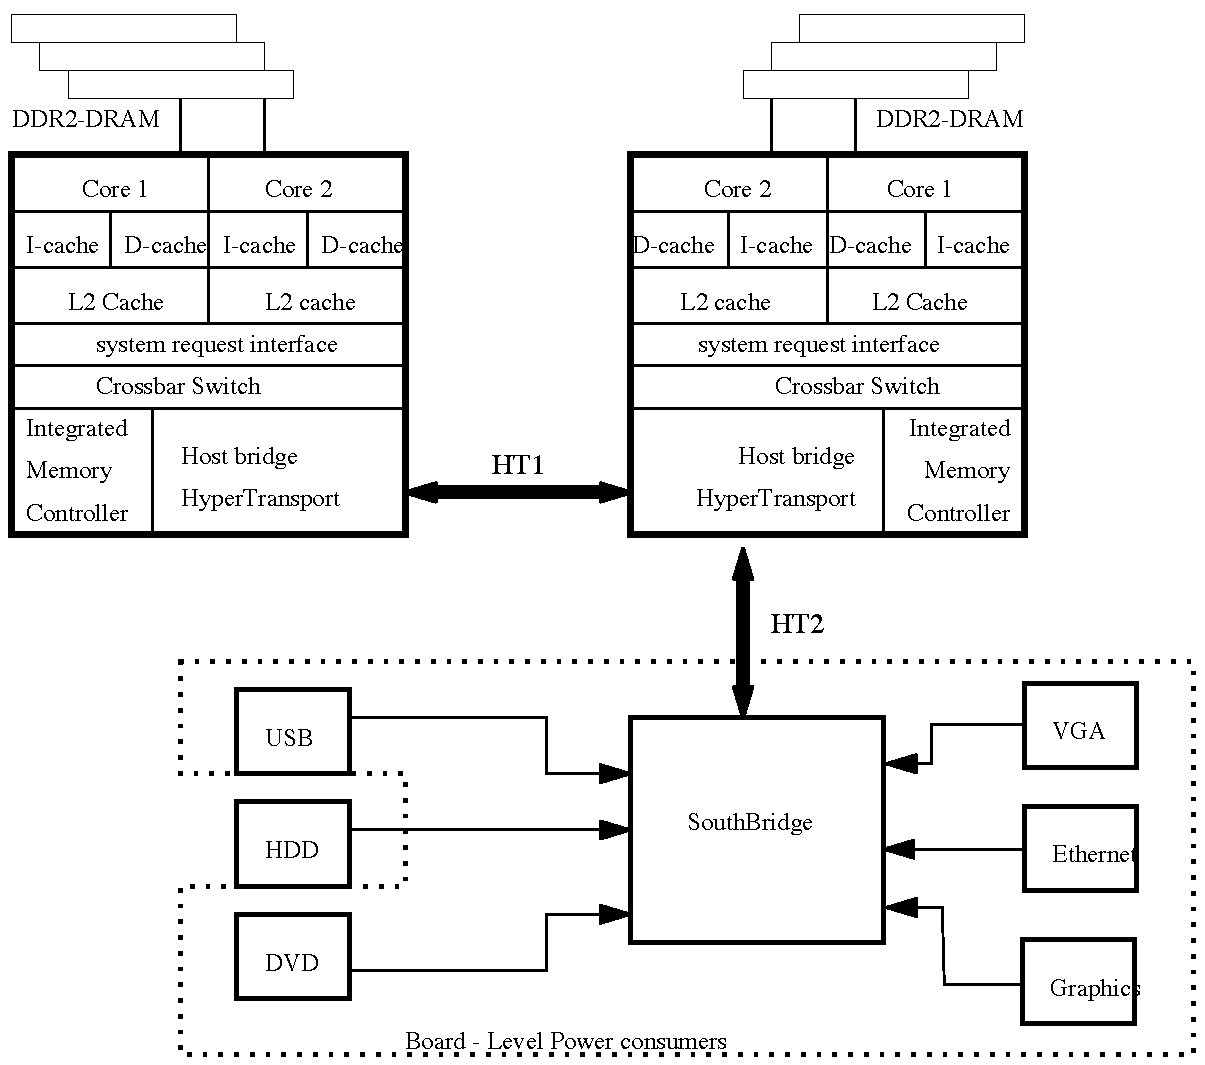
\includegraphics[scale=0.3]{x2200sys}
     \caption{AMD Opteron architecture.}
     \label{fig:amdarch}
  \end{minipage}\hspace{0.1cm}
  \begin{minipage}{0.5\linewidth}
  \centering
     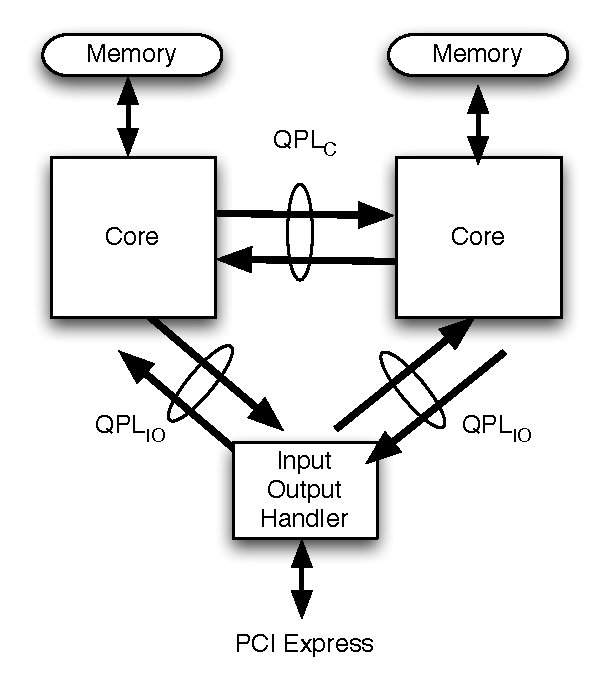
\includegraphics[scale=0.5]{intelnehalem}
     \caption{Intel Xeon (Nehalem) architecture.}
     \label{fig:intarch}
  \end{minipage}
\end{figure*}
\section{Processor energy consumption}
\label{sec:procmodel}
Consider the AMD Operton architecture and the Intel Nehalem
architecture, as depicted in \figurenames~\ref{fig:amdarch} and
\ref{fig:intarch}.  The former is a NUMA-based processor
(\figurename~\ref{fig:amdarch}), with Northbridge functionality
incorporated in the processor core and each core responsible for local
access to the memory connected to that Northbridge logic (shown in
\figurename~\ref{fig:amdarch} as ``Integrated Memory Controller'').
Processor cores on a single die are connected via a crossbar to the
HyperTransport bus (i.e., HT1) between processors.  A coherent bus
protocol is used to ensure memory consistency between processor cores on
each die.  In addition, the master processor in the system is connected
via a second HyperTransport bus (i.e., HT2) to the Southbridge device
that manages connections to the outside world.  A similar structure
exists in the Intel Xeon Nehalem architecture.  Unlike the AMD Operton,
each Nehalem processor is connected to an Input-Output handler, which
provides the Southbridge with connecting functions for off-chip resources.

It is observed that work done by any of the processors, as the heart of
energy consumption in a server system, can be quantified in terms of bus
transactions in and out of the processors.  Traffic on the external
buses provides a measure of how much data is processed by the processor.
Our energy consumption model aims to treat each processor as a black
box, whose energy consumption is a function of its work load (as
manifested by core die temperatures measured at the system level by
\texttt{ipmitool} through sensors on the path of the outgoing airflow
from the processor).  In practice, when estimating processor power
consumption based on PeCs (performance counters), there are only a
limited number of PeCs for tools, like \texttt{cpustat}, to track simultaneously.

For the AMD dual-core Operton architecture (shown in
\figurename~\ref{fig:amdarch}), traffic on the HT buses is viewed as a
representative of the processor workload, reflecting the amount of data
being processed by a processor (i.e., its involved cores).  The HT2 bus
is non-coherent and connects one of the two processors to the
Southbridge (whereas the Northbridge is included on the Opteron
processor die).  Thus, traffic on the HT2 bus reveals hard-disk and
network transactions.  This model scales by considering the effect of
network traffic and disk I/O transactions.  HT1 is a coherent bus
between the two SMP processors and, as such, PeCs on HT1 provide
accurate estimation on the processing load of cores executing jobs.
Per-core die temperature readings are directly affected by the number of
transactions over the HT1 bus.  A similar observation holds for the QPL
links present in the Intel Nehalem architecture, with traffic between
its two cores reflected by transactions on QuickPath Links between the
cores, denoted by $QPL_C$ (see \figurename~\ref{fig:intarch}).

Therefore, total processor power consumption at time $t$, $P_{proc}(t)$,
is related to processor temperature readings and the estimated amount of
data being processed at the time, and it can be expressed as a function
of three metrics: die temperature readings for processors 0 and 1, and
the number of bus transactions (i.e., traffic over HT1 for the AMD
server and over $QPL_C$ for the Intel server).  We have processor energy
consumption between times $t_{1}$ and $t_{2}$ as follows:
\begin{equation}
  \label{eq:procpwr2}
  E_{proc}=\displaystyle\int_{t_{1}}^{t_{2}}\left( {P_{proc}(t)} \right)dt.
\end{equation}
\section{DRAM energy consumption}
\label{sec:dram}
Energy consumed by the DRAM banks is directly related to the number of
DRAM read/write operations involved during the time interval of
interest, and the number is reflected by (1) the last-level cache misses
for all $N$ constituent cores ($CM_{i}(t)$, $i$ = 1, 2, ..., $N$) in
the server when executing jobs and (2) the data amount due to disk
accesses for OS support (like page tables, checkpoints, virtual
environments) and due to performance improvement for peripheral devices
(like buffered data for disks and optical devices, spooled printer
pages).  The data amount in (2) above, named $DB(t)$, is reflected by
traffic over $HT_{2}$ (or QuickPath links between the two cores and the
Input/Output handler, denoted by $QPL_{IO}$) for the AMD Opteron server
(or the Intel Xeon server), as demonstrated in
\figurename~\ref{fig:amdarch} (or \figurename~\ref{fig:intarch}).
This is because network traffic does not exist in either testing server,
which comprises only a single chip.  Additional energy contributors
include activation power and DRAM background power (due to leaking
currents), represented by $P_{ab}$.  As stated earlier
\cite{Micron2007}, DRAM activation power and background power can be
obtained from the DRAM documentation, and they together amount to 493 mW
for one DRAM module in our AMD Opteron server.  Consumed energy over the
time interval between $t_{1}$ and $t_{2}$ can be expressed by
\begin{equation*}
  \label{eq:dram}
  E_{mem}=\displaystyle\int_{t_{1}}^{t_{2}}\left( (\sum_{i=1}^{N}CM_{i}(t)+DB(t))\times
    P_{DR}+P_{ab}\right)dt,
\end{equation*} 
where $P_{DR}$ refers to DRAM read/write power per unit data.
\begin{table}[tp]
\caption{Hitachi HDT725025VLA360 disk power parameters}
\centering
\begin{tabular}{ l l }
\hline
\textbf{Parameter} & \textbf{Value} \\
\hline
  Interface & Serial ATA\\
  Capacity & 250 GB\\
  Rotational speed & 7200 rpm  \\
  Power & \\
  ~~Spin up& 5.25 W (max)\\
  ~~Random read, write & 9.4 W (typical)\\
  ~~Silent read, write & 7 W (typical)\\
  ~~Idle & 5 W (typical)  \\
  ~~Low RPM idle & 2.3 W (typical for 4500 RPM)\\
  ~~Standby & 0.8 W (typical)\\
  ~~Sleep & 0.6 W (typical)\\
\hline
\end{tabular}
\label{tab:hddparam}
\end{table}
\section{Hard disk energy consumption}
\label{sec:networkengery}
Energy consumed by the hard disk(s) is approximated by using a
combination of relevant PeCs and drive ratings.  Both our test servers
use the Hitachi's SATA hard disk (whose specification and relevant power
consumption figures are listed in Table ~\ref{tab:hddparam}).  Based on
the physical, electrical, and electromechanical parameters of a hard
disk, one can construct its detailed power consumption model.  However,
a cruder but simpler model can be obtained from the typical power
consumption data of hard disks and pertinent PeCs, including (1) the
number of reads and writes per second to the disk and (2) the amount of
data (in kilobytes) read from and written to the disk.  Those PeCs can
be measured by the tool of \texttt{iostat}, arriving at approximate disk
power consumption, $E_{hdd}$, as:
\begin{align*}
\label{eq:hddpwr1}
E_{hdd} = &P_{spin-up}\times T_{su}+  P_{read}\sum N_r\times T_r \nonumber\\
        &+ P_{write}\sum N_w\times T_w+ \sum P_{idle}\times T_{id}
\end{align*}
where $P_{spin-up}$ is the power required to spin-up the disk from 0 to
full rotation, and $T_{su}$ is the time required to achieve spin up,
typically about 10 sec.  $P_{read}$ (or $P_{write}$) is the power
consumed per kilobyte of data read from (or written to) the disk,
whereas $N_r$ (or $N_w$) is the number of kilobytes of data reads (or
data writes) in time-slice $T_r$ from (or to) the disk.  The Hitachi
disk achieves read operations at 1.5 Gbits/s, when consuming 530 mA
current at +5V, thereby exhibiting approximately $13.3 \mu W$/Kbyte.
Similarly, it is found to consume $6.67 \mu W$/Kbyte for write
operations.  The numbers of $N_r$ and $N_w$ can be obtained using
\texttt{iostat} according to the chosen time slice.

There are two idle states for the disk: idle and unloaded idle (when
disk read/write heads are unloaded).  The time to go from the unloaded
idle state to the idle state is usually less than 1 second (smaller than
the resolution of \texttt{iostat}).  Thus, a history match count in the
\texttt{iostat} statistics with zero reads and writes signifies the
periods in which the disk is idle, permitting us to compute idle energy
consumption accordingly.  \texttt{iostat} readings for the durations of
switching to different disk power states may be obtained with a more
in-depth analysis, which is not consider in this work.
\section{Board energy consumption}
\label{sec:board}
The quantity of $E_{board}$ represents energy consumption caused by the
support chipsets, control logic, buses, signal links, etc.,
and it usually falls into the 3.3V and 5V power domains.
In our case, this value is obtained using current probe-based measurements.
The results measured over an interval of interest, $t_{interval}$,
excluded the effects of processor, disks, fans, and optical devices, leading to:
\begin{equation}
\label{eq:board}
E_{board} = \left(\sum V_{power-line}\times I_{power-line}\right) \times t_{interval}.
\end{equation}
Note that introducing the current sensors (possibly taking up to 28 for
a server ~\cite{SSI2004}) to the power lines on the board will provide
instantaneous current readings for use in \equationname~(\ref{eq:board}).

Aggregated power consumption effects on the board may be captured using
ambient temperature readings on the board.  Such readings can be
obtained using system management tools commonly found in server
environments (such as IPMI), and they are included in the set of our PeCs
for energy consumption estimation.
\section{Electromechanical energy consumption}
\label{sec:electrical}
A server always involves electromechanical energy consumption, $E_{em}$,
which is mainly due to the electromechanical functions related to system
cooling.  Multiple fans often exist in a server for cooling.  Power
drawn by the $i^{th}$ fan at time $t$ can be given by the following
equation:
\begin{equation}
\label{eq:fanp}
P_{fan}^{i}(t) = P_{base} \times \left(\frac{RPM_{fan}^{i}(t)}{RPM_{base}}\right)^3
\end{equation} 
where $P_{base}$ defines the base power consumption of the unloaded system
when running only the base operating system and no application workload.
The $P_{base}$ value is obtained experimentally by measuring the current drawn
on the +12V and +5V lines, using a current probe and an oscilloscope.
There is a current surge at system start, which is neglected.
Under nominal conditions, the +12V line draws approximately 2.2A
to power both blower fans in the AMD testing server.

A server with $N$ cooling fans results in electromechanical power at time $t$ as
\begin{equation*}
\label{eq:electp}
P_{elect}(t) =  V(t) \cdot I(t) + \sum_{i=1}^NP_{fan}^{i}(t)
\end{equation*} 
where the first term is instantaneous DC power output from the power supply,
representing DC power consumed by the server, and
$P_{fan}^{i}(t)$ is expressed in \equationname~(\ref{eq:fanp}).

Total electromechanical energy consumption over a given task execution
period of $T_{p}$ equals:
\begin{equation*}
\label{eq:elect}
E_{em} =  \int^{T_{p}}_0 \left(V(t) \cdot I(t) + \sum_{i=1}^NP_{fan}^{i}(t)\right)dt.
\end{equation*} 
\begin{figure}[tp]
\begin{center}
     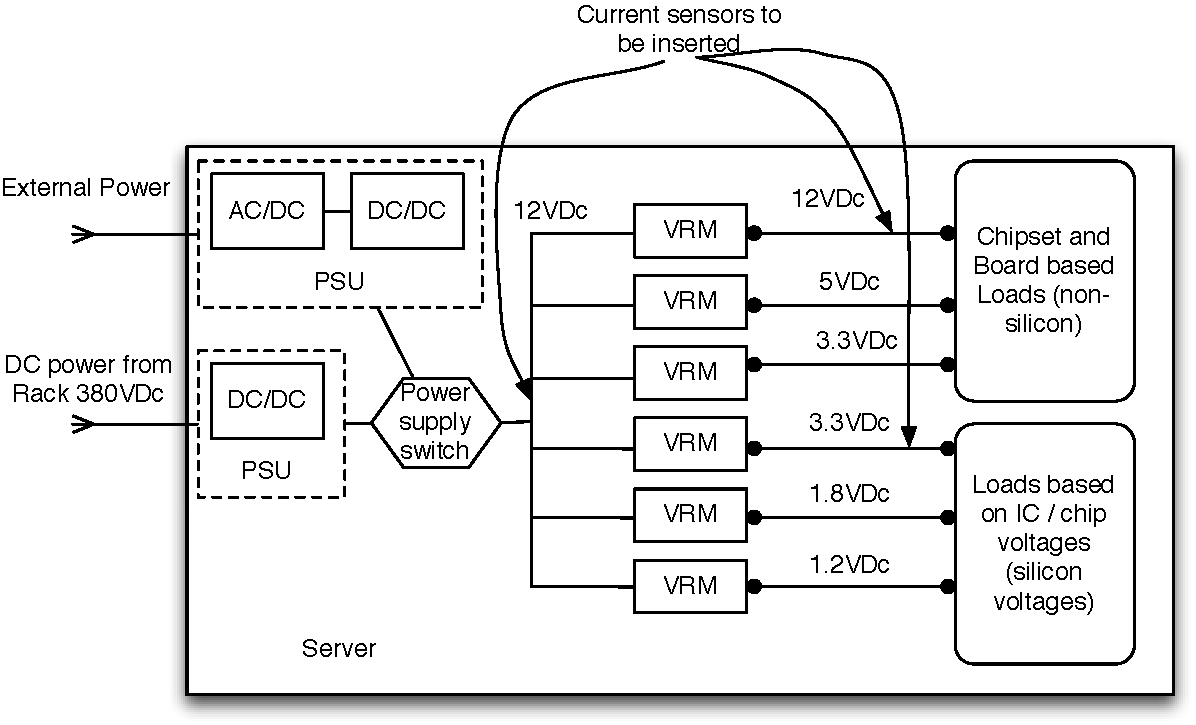
\includegraphics[scale=0.60]{acdcpower2.pdf}
     %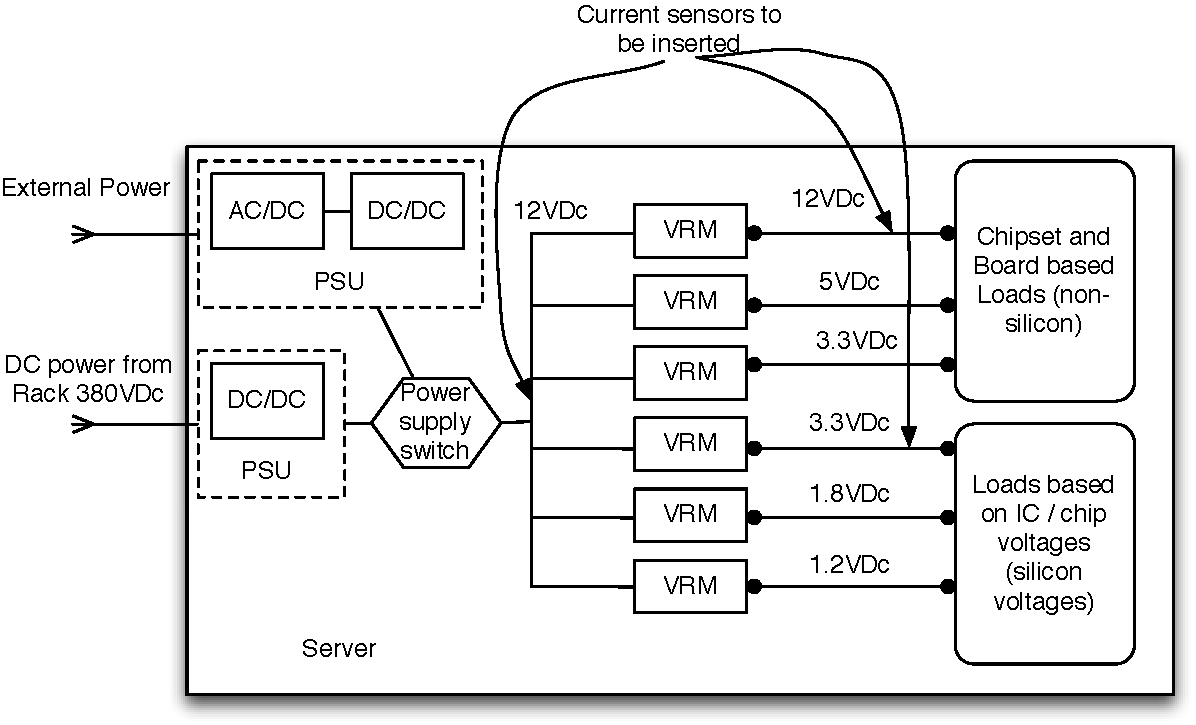
\includegraphics[]{acdcpower2.pdf}
     \caption{Proposed power distribution for servers.}
     \label{fig:psu}
\end{center}
\end{figure}
\section{Proposed power distribution}
\label{sec:powerdist}
The input to our derived energy consumption model is current readings at
the power supply lines to the server components.  While not available
yet, current sensors (like MAXIM's 4473~\cite{maxim2006}) may be placed
at the outputs of the power supply unit (PSU, see
\figurename~\ref{fig:psu}) to dynamically track DC power draws during
job execution as system load varies.  A power distribution diagram, with
current sensors incorporated as measurable PeCs, is depicted in
\figurename~\ref{fig:psu}, where a rack-level DC power source is used
for power savings due to its better power efficiency.

With current sensors provided at the output of the DC voltage lines
delivering power to the hard disk drives, for example, one may measure
hard disk power consumption in real-time.  Let the current sensors at
+5V (or +12V) lines to the hard disk be denoted by $v_1(t)$ and $i_1(t)$
or ($v_2(t)$ and $i_2(t)$), which is no larger than 730mA (or 630mA),
we have $E_{hdd}$ as follows:
\begin{equation*}
\label{eq:hddpwr2}
E_{hdd} =  \int_{t1}^{t2} \left( v_1(t)\times i_1(t) + v_2(t)\times i_2(t) \right) dt.
\end{equation*}
Given no current sensors available in our experimental servers, we
obtained the readings by a current probe, logged through an
oscilloscope.

Typically, a server at the idling state (when running the operating
system and no application jobs) consumes some 40 to 42\% of its rated
power (which is 450W in our case).  Conversion efficiency increases to
about 80\% when the server is heavily loaded, and the SMPS regulates the
power supply to work at 75\% conversion efficiency when power drawing is
over 50\% of the rated one.  Hence, conversion losses of the power
supplied to the system is at least 20\%, even for the best conversion
scenario.  Earlier studies \cite{ton2008} have shown that most DC
systems perform better in terms of power efficiency than their AC
counterparts.  A typical AC-based server system has a power supply
efficiency of 73\%, as compared with a 92\% for a DC system.  Also, the
overall system efficiency for an AC system is 61\%, in comparison to
85\% for a DC system.

While a rack level DC power distribution system easily translates into
large power savings at the server level, our model considers a part of
this power conversion unit, since it is not software tunable in its
present state. Currently, our model externally monitors the input power
to the system and controls the power, and consequently, thermal envelope
of the system, based on the processing load.

To understand how our analytical model can be improved by the addition
of such sensors (as valuable PeCs), consider how one might partition
$E_{dc}$ by having access to this information.  Most power supplies
limit the total power delivered through the 5V and 3.3V lines to about
20\% of the rated power supply ($P_R$).  Assuming that each of the
voltage lines in domain $j$, $v_{k}^{j}(t)$, draws current
$i_{k}^{j}(t)$, then each line draws instantaneous power of
$p_{k}^{j}(t) = v_{k}^{j}(t)\cdot i_{k}^{j}(t)$.  Given a voltage domain
with $M_{j}$ DC lines as output, the total power delivered for voltage
domain $j$ is:
\begin{equation*}
\label{eq:power_vdomain}
p_{v}^{j}(t)=  \sum_{k=1}^{M_{j}} v_{k}^{j}(t)\cdot i_{k}^{j}(t)
\end{equation*}

If the board has $N$ voltage domains: $v_{1}$, $v_{2}$, $\ldots$, $v_{N}$,
total DC power delivered into the system equals:
\begin{align*}
\label{eq:power_vtot}
p_{dc}(t) = \sum_{j=1}^{N} p_{v}^{j}(t)\\
         =  \sum_{j=1}^{N} \sum_{k=1}^{M_{j}} v_{k}^{j}(t)\cdot i_{k}^{j}(t).
\end{align*}
Total energy delivered to the system between times $t_2$ and $t_1$ is:
\begin{equation*}
\label{eq:power_input}
E_{dc} = \int_{t_1}^{t_2} p_{dc}(t) dt  = \int_{t_1}^{t_2} \sum_{j=1}^{N} \sum_{k=1}^{Mj} v_{k}^{j}(t)\cdot i_{k}^{j}(t) dt.
\end{equation*}
\clearpage
For the 3.3V and 5V lines, we have the following constraint:
\begin{align*}
\label{eq:power_constr}
E_{dclv} &= \int_{t_1}^{t_2} p_{dclv} (t) dt \nonumber\\
        &=  \int_{t_1}^{t_2} \left( \sum_{k=1}^{M_{1}} v_{k}^{1}(t)\cdot i_{k}^{1}(t) +
        \sum_{k=1}^{M_{2}} v_{k}^{2}(t)\cdot i_{k}^{2}(t) \right) dt \nonumber\\
        & \leq 0.2 P_R
\end{align*}
where $M_{1}$ and $M_{2}$ are the total 3.3V and 5V lines, respectively.
Thus, in our 450W rated system, the power delivered by the 3.3V and 5V lines is capped at 90W.

\section{Thermal  Extensions to the Model}
\label{sec:themalmodel}
There are two metrics of interest for the thermal workload of a
multi-core processor. An application $A$ has a length $L(A,D_{A},t)$
which is the total time of execution $t$ of
the application working upon a set of data $D_{A}$. The
application $A$ is composed of $p$ processes, with each process
associated with a data set of size $d_i$, for $1\leq i \leq p$, in a
single logical CPU. The total data associated with an application $A$ is
the sum of the data associated with its component processes:
\begin{equation}
\label{eq:totaldata}
D_{A}=\displaystyle\sum_{i=1}^p{d_i}.
\end{equation}
We assume that the activities are taking place in a staging area which
contains the main and virtual memory operating spaces, as well as the
processor with its cores and their associated caches and shared cache.
This time of execution measurement includes both computation time and
the time to move the data for the problem from the staging area
(peripherals off the chip like DRAM and HDD) to a computation or
operation area (on the chip such as the caches and the cores).

The second metric of interest is the energy consumption or energy
workload of an application, $U(A,D_{A},t)$. For each application $A$ and
problem size $D_{A}$, we define the the workload $W(p_{i},d_{i},t)$, $1
\leq i \leq p$, in a data-operation dependent and system-independent
way. The workload $W$ contains two components: (1) the operations
count that is performed by the computational core, and (2) the
communication operations required for transfer of data, instructions, and data
coherency and book-keeping operations. These are measured in terms of
the number of bytes operated upon, or number of bytes transferred. Thus
the energy workload of an application $A$ operating on a data set $D_A$
can be expressed as:
\begin{equation}
\label{eq:eworkload}
U(A,D_{A},t) = \displaystyle \lim_{n \to k_e }n \times W(p_i,d_i,t)
\times L_n(A_{n},D_{A_{n}},t), 1\leq i \leq p
\end{equation}
where $L_n(A_{n},D_{A_{n}},t)$ is the total time to execute $n$ applications using
the chip. The term $k_{e}$ is the total number of applications that can be
executed with the associated length of time for $L_n$, at which point a
``thermal event'' will occur causing the applications and the system to
catastrophically fail, or shut down.

It is easy to see that the above term is energy consumption of the
system till a thermal event occurs. In order to relate the energy
expenditure of the system while running applications, to the
corresponding joule heating, we define the term ``Thermal Equivalent of
Application\index{idx:tea}'' (TEA), which is defined as the electrical work converted
to heat in running an application and is measured in terms of die
temperature change and ambient temperature change of the system. Thus for
the application $A$ we express TEA as :
\begin{equation}
\label{eq:tea}
\Theta_A(A,D_{A}, T,t) = \frac{U(A,D_{A},t)}{\displaystyle \lim_{T \to T_{th}} J_e \times (T - T_{nominal})}
\end{equation}
The quantity $T_{th}$ refers to the threshold temperature at which a DTM
triggered event will occur.  $T_{nominal}$ refers to the nominal
temperature as reported by the DTM counters/registers when the system is
in a quiescent state, i.e., only the operating system is running and no
application is being executed. The term $J_{e}$ is the ``electrical
equivalent of heat'' for the chip, which reflects the
\textit{informational entropy}\index{ientropy} of the system associated with processing
the data bits that application $A$ computes and communicates, as well as
the black body thermal properties of the chip packaging and the cooling
mechanisms around the chip. Thus, TEA is a dimensionless quantity with
both denominator and numerator expressing work done or energy consumed
in finishing a task.

For managing the thermal envelope of applications on server systems as
well as embedded systems, we are interested in the thermal efficiency of
the operation, that is, the thermal cost of taking an application to
completion. The thermal efficiency is defined as:
\begin{equation}
\label{eq:thermeff}
\eta(A, D_{A},T,t) = \frac{\Theta_A(A,D_{A}, T,t)}{\Theta_A(A_e,D_{A_{e}}, T_{me}, L_{e})}
\end{equation}
where $T_{me}$ is the maximum temperature which the core will carry
over until a DTM triggered event occurs and $A_e$ refers to the application
whose energy consumption has caused the DTM triggered event to take
place. $L_{e}$ is the execution time of application $A_e$. Thus
$\eta(A, D_{A},T,t)$ is a measure of the ``thermal efficiency of the
application'', which implies how much an application affects temperature
change without compromising it's throughput and/or leads to a thermal
event. Thus the definition of $\eta$ is linked to the definition of the
thermal and energy workload.

We combine these metrics into the achieved performance per unit power
consumed by the chip:
\begin{equation}
\label{eq:thermcost}
C_{\theta}(A, D_{A}, T,t)=\frac{\Theta_A(A,D_{A}, T, t)}{E_{sys}(A,D_{A},t)}
\end{equation}
where $E_{sys}(A,D_{A},t)$ is the overall power consumed during the
application lifetime.  We can apply \equationname~\ref{eq:linmodel} to
\equationname~\ref{eq:thermcost} to apportion the total power consumed
by a single physical component (processor, DRAM units, HDD, motherboard,
and electrical/electromechanical) during the length $L_{A}$ of the
application.

This normalized quantity $C_\theta$ gives some indication of the
``cost'' of executing an application on the given chip.  The problem of
application scheduling requires that we find the best application
ordering that minimizes:
\begin{equation}
\label{eq:thermopt}
  \frac{\partial^{2} C_{\theta}(A, D_{A}, T, t)}{\partial T \partial t}
  =
  \frac{\partial^{2}}{\partial T \partial t}
  \left(
  \Theta_{A}(A,D_{a},T,t)
  \times
  C_{\theta}(A, D_{A}, T,t)
  \right).
\end{equation}

% Following comment block used by GNU-EMACS and AUCTEX packages
% Please do not remove.
%%% Local Variables: 
%%% mode: latex
%%% TeX-master: "prospectus.tex"
%%% End: 

% 
% File:    chapter-prediction.tex
% Author:  awl8049
% Revision:$Revision: 1.4 $
%
\chapter{Effective Prediction}
\label{chp:application}
The current generation of server systems lacks (1)~the complete set of
measurement and monitoring capabilities and (2)~data flow state capture
mechanisms required in order to formulate the parameters of an exact
analytical model.  For example, the system board DC and AC power
consumption cannot be easily split in measurements or analyses, due to
the presence of large numbers of voltage/current domains, each with
multiple components.  Therefore, effective prediction on future power
consumption and temperature changes based on past reading/measurements
(obtained from PeCs and performance metrics) is critical.

In \equationname~(\ref{eq:linmodel}), $E_{system }$ signifies total
energy consumed by the system for a given computational workload, equal
to the sum of five terms: $E_{proc}$, $E_{mem}$, $E_{hdd}$, $E_{board}$,
and $E_{em}$.  Adopting \equationname~(\ref{eq:linmodel}) for server
energy consumption estimation, one needs to predict change in
$E_{system}$ over the time interval of $(t, t+\Delta t)$.  Such
prediction, following a time series to make observations of the server
system, based on PeCs and performance metrics, can be approximated by
\begin{equation}
\label{eq:tseries}
E_{system} = \hat{f}(E_{proc}, E_{mem}, E_{hdd}, E_{board}, E_{em}),
\end{equation}
where the involved parameters correspond to the five server energy
contributors modeled in Sections~\ref{sec:procmodel} to \ref{sec:electrical}.
\section{Performance counters and metrics}
\label{sec:variables}
In our prediction approach, fourteen (14) observable PeCs and accessible
performance metrics (referred to as "measures" collectively for simplicity)
are involved in the AMD server, as listed in Table~\ref{tab:model}.
They are grouped into five clusters, depending on their relevance to the
server energy contributors.  More specifically, the top three measures
are related to $E_{proc}$, named $MP_{proc}^{AMD} = \left[T_{C_{0}},
  T_{C_{1}}, HT_{1}\right]$.  The next five measures dictate $E_{mem}$,
denoted by $MP_{mem}^{AMD} = \left[HT_{2}, CM_{0}, CM_{1}, CM_{2},
  CM_{3}\right]$.  Those $CM_i$ measures, capturing the total L2 cache
miss counts due to Core $i$, are registered at \texttt{PAPI\_L2\_TCM} (being
OpenSolaris generic events equivalent to the matching event in the Linux
PAPI performance counter library \cite{London2001}) and mapped to the
AMD performance counters at 0x7E (as defined in \cite{AMD2008}).  The
following two measures are pertinent to $E_{hdd}$, represented by
$MP_{hdd}^{AMD} = \left[D_{r}, D_{w}\right]$, which refer to the total
numbers of bytes in disk reads and disk writes, respectively, during a
period of 5 seconds (in our experiments) for all I/O devices (which are
limited to the disk only, since no network traffic nor optical disks
exist in the two testing servers), as recorded by the system activity
monitor.  The next two measures are related to $E_{board}$, indicated by
$MP_{board}^{AMD} = \left[T_{A_0}, T_{A_1}\right]$, which register the
temperature readings of two board locations where temperature sensors
are placed.  Finally, the last two measures determine $E_{em}$, shown by
$MP_{em}^{AMD} = \left[F_C, F_M\right]$, which provide speed information
of the CPU cooling fan and the memory cooling fan.  Collectively, each
observation at time $t$ includes the 14 measures of $MP^{AMD}(t) =
\left[MP_{proc}^{AMD}, MP_{mem}^{AMD}, MP_{hdd}^{AMD},
  MP_{board}^{AMD},MP_{em}^{AMD}\right]^{T}$.
\begin{table}[t!]
  \caption{PeCs and performance metrics for AMD Opteron server}
  \label{tab:model}
  \centering
  \begin{tabular}{r l}
\hline
\textbf{Variable}&\textbf{Measurement}\\
\hline
$T_{C_{0}}$&CPU0 Die Temp\\
$T_{C_{1}}$&CPU1 Die Temp\\
$HT_{1}$&HT1 Bus X-Actions\\
$HT_{2}$&HT2 Bus X-Actions\\
$CM_{0}$&Last-level Cache Misses due to Core0\\
$CM_{1}$&Last-level Cache Misses due to Core1\\
$CM_{2}$&Last-level Cache Misses due to Core2\\
$CM_{3}$&Last-level Cache Misses due to Core3\\
$D_{r}$&Disk bytes read\\
$D_{w}$&Disk bytes written\\
$T_{A_{0}}$&Ambient Temp0\\
$T_{A_{1}}$&Ambient Temp1\\
$F_{C}$&CPU Cooling Fan Speed\\
$F_{M}$&Memory Cooling Fan Speed\\
\hline
  \end{tabular}
\end{table}
\begin{table}[t!]
  \caption{PeCs and performance metrics for Intel Nehalem server}
  \centering
  \label{tab:intelmodel}
  \begin{tabular}{r l}
\hline
\textbf{Variable}&\textbf{Measurement}\\
\hline
$T_{C_{0}}$&CPU0 Die Temp\\
$T_{C_{1}}$&CPU1 Die Temp\\
$QPL_{C}$&Transactions on QPL between Cores\\
$QPL_{IO}$&Transactions on QPLs for IO Handler\\
$CM_{0}$&Last-level Cache Misses due to Core0\\
$CM_{1}$&Last-level Cache Misses due to Core1\\
$D_{r}$&Disk bytes read\\
$D_{w}$&Disk bytes written\\
$T_{A_{0}}$&Ambient Temp0\\
$T_{A_{1}}$&Ambient Temp1\\
$T_{A_{2}}$&Ambient Temp2\\
$F_{C}$&Memory Cooling Fan Speed\\
$F_{M2a}$&Memory Cooling Fan Speed 2a\\
$F_{M2b}$&Memory Cooling Fan Speed 2a\\
$F_{M3a}$&Memory Cooling Fan Speed 3a\\
$F_{M3b}$&Memory Cooling Fan Speed 3b\\
$F_{M4a}$&Memory Cooling Fan Speed 4a\\
$F_{M4b}$&Memory Cooling Fan Speed 4b\\
$F_{M5a}$&Memory Cooling Fan Speed 5a\\
$F_{M5b}$&Memory Cooling Fan Speed 5b\\
\hline
  \end{tabular}
\end{table}

On the other hand, the Intel Nehalem server involves nineteen (19) measures, as
listed in Table~\ref{tab:intelmodel}.  Again, they are classified into five
groups, each associated with one server energy contributor.
Notice that $QPL_{C}$ and $QPL_{IO}$ are relevant to QuickPath Links
(depicted in \figurename~\ref{fig:intarch}),
and they are associated with $E_{proc}$ and $E_{mem}$, respectively.
In practice, however, there is just one single PeC for holding aggregated
$QPL_{C}$ and $QPL_{IO}$ together.
Among those measures listed in Table~\ref{tab:intelmodel},
the top three are pertinent to $E_{proc}$, comprising $MP_{proc}^{Intel}$.
The next three measures determine $E_{mem}$, forming $MP_{mem}^{Intel}$.
Those two $CM_{i}$ measures indicate the total L3 cache miss counts
due to Core \textit{i}, $i$ = 0 or 1.
The cache miss counts record the last-level cache (i.e., L3) misses
for the Intel Xeon processor on which our testing Intel
server is built.  They are reflected by the OpenSolaris generic event,
\texttt{PAPI\_L3\_TCM} (as detailed in \cite{Sun2008b} and \cite{Intel2009}).
The next two measures are related to $E_{hdd}$ (and constitute $MP_{hdd}^{Intel}$),
signifying the total numbers of bytes in disk reads and disk writes,
respectively, during a period of 5 seconds.
The subsequent three measures dictate $E_{board}$, obtained
from 3 temperature sensors placed on the board for ambient temperature readings;
they form $MP_{board}^{Intel}$.
Finally, the last nine measures determine $E_{em}$, offering speed
information of those nine memory cooling fans, to constitute $MP_{em}^{Intel}$.
As a result, each observation for the Intel server at time $t$ comprises the 19 measures of
$MP^{Intel}(t) =\left[MP_{proc}^{Intel}, MP_{mem}^{Intel}, MP_{hdd}^{Intel}, MP_{board}^{Intel}, MP_{em}^{Intel}\right]^{T}$.

A common prediction approach follows the linear auto-regressive (AR)
combination of observation measures to predict the quantities in
\equationname~(\ref{eq:tseries})  \cite{Lewis2008}.
It yields $E_{system}$ by adding up $f_{co}(MP_{co})$ for all server energy
contributors, with each $f_{co}$ (due to Contributor $co$) being a
linear summation of its constituent measures, as detailed in Appendix.
Such a linear AR approach has characteristics that make it unsuitable
for modeling server systems.  Consider the traces of actual power shown
in \figurenames~\ref{fig:compareamd} and \ref{fig:compareintel} for the
SPEC CPU2006 zeusmp benchmark as executed on an AMD Opteron or Intel
Nehalem server.  We saw indications of (1) periodic behavior and (2)
large swings in the power draw throughout the course of the benchmark run.
Similar scenarios were observed for other benchmarks on 
the AMD Opteron server and the Intel Nehalem server under this work.
Linear regression-based prediction for power draw can
mis-predict substantially (up to 44\%, as indicated in
Table~\ref{tab:modelerroroptIntel}).  Thus, it is reasonably conjectured
that \textit{non-linear dynamics} do exist in server systems.  Given
large swings in power draw usually occur to a typical server and cannot
be completely attributed to noise, more accurate prediction than linear
auto-regression and MARS \cite{Friedman1991} is indispensable.
\section{Chaotic prediction}
\label{sec:chaospredict}
The continuous system expressed in \equationname~(\ref{eq:linmodel}) can
be viewed as a multi-variate differential equation in the time domain
(energy being power used in a time period).  The time series
approximation of a system solution can be viewed as a projection of
the flow of \equationname~(\ref{eq:linmodel}) onto a surface~\cite{Liu2010}.
The projection is defined in a way that the behavior (i.e., energy consumption)
of the dynamic system is reflected in our discrete approximation
(i.e., our time series measures).

We performed an analysis on the data collected from our test systems to
determine if the behavior of our time series can be attributed to some
form of chaotic behavior.  A chaotic process is one which is highly
sensitive to a set of initial conditions.  Small differences in those
initial conditions yield widely diverging outcomes in such chaotic
systems.  In order to determine whether a process is chaotic, we must be
able to show that (1) it demonstrates high sensitivity to initial
conditions and topological mixing, and (2) its periodic orbits are dense
\cite{Sprott2003}.  After analyzing our experimental data, we believe
that the power consumption of a server demonstrates \textit{chaotic behavior}.

In order to evaluate a server's sensitivity to initial conditions, we
consider the Lyapunov exponents of the time series data observed while
running those benchmarks described in the previous section.  The
Lyapunov exponent quantifies the sensitivity of a system such that a
positive Lyapunov exponent indicates that the system is chaotic
\cite{Sprott2003}.  The average Lyapunov exponent can be calculated using
$\lambda = \displaystyle\lim_{N\to\infty}\frac{1}{N}\sum_{n=0}^{N-1}ln|f'(X_n)|$.

We found a positive Lyapunov exponent when performing this calculation
on our data set, ranging from 0.01 to 0.28 (or 0.03 to 0.35) on the AMD
(or Intel) test server, as listed in Table~\ref{tab:chaotic}, where
each pair indicates the parameter value of the AMD server followed by
that of the Intel server.  Therefore, our data has met the first and
the most significant criterion to qualify as a chaotic process.

The second indication of the chaotic behavior of the time series in
\equationname~(\ref{eq:tseries}) is an estimate of the Hurst parameter
$H$ for the data sets collected in each benchmark.  A real number in the
range of $(0, 1)$, the Hurst parameter is in the exponents of the
covariance equation for Fractional Brown motion (fBm) \cite{Sprott2003}.
If the value of the Hurst parameter is greater than $0.5$, an increment
in the random process is positively correlated and long range dependence
exists in the case of time series.  In a chaotic system, a value of $H$
approaching 1.0 indicates the presence of self-similarity in the system.
As demonstrated in Table~~\ref{tab:chaotic}, the time series data
collected in our experiments all have values of $H$ close to 1.0,
ranging from 0.93 to 0.98 (or 0.93 to 0.97) on the AMD (or Intel) test
server.
  \begin{table}[t!]
    \caption{Indications of chaotic behavior in power time series (AMD, Intel)}
    \label{tab:chaotic}  
    \centering
    \begin{tabular}{c  r r r }
      \hline
      \multicolumn{1}{c }{\textbf{Benchmark}}&\multicolumn{1}{c}{\textbf{Hurst}}&&\multicolumn{1}{c}{\textbf{Average}}\\
      \multicolumn{1}{c }{~}&\multicolumn{1}{c}{\textbf{Parameter}}&&\multicolumn{1}{c}{\textbf{Lyapunov}}\\
      \multicolumn{1}{c }{~}&\multicolumn{1}{c}{($H$)}&&\multicolumn{1}{c}{\textbf{Exponent}}\\
      \hline
      bzip2    &(0.96, 0.93)&&(0.28, 0.35)\\
      cactusadm&(0.95, 0.97)&&(0.01, 0.04)\\
      gromac   &(0.94, 0.95)&&(0.02, 0.03)\\
      leslie3d &(0.93, 0.94)&&(0.05, 0.11)\\
      omnetpp  &(0.96, 0.97)&&(0.05, 0.06)\\
      perlbench&(0.98, 0.95)&&(0.06, 0.04)\\
      \hline
    \end{tabular}
\end{table}

From a predictive standpoint, the unpredictable deterministic behavior
of chaotic time series means that it is difficult to build a predictor
that takes a global parametric view of the data in the series.  However,
it is possible to generate a highly accurate short-term prediction by
reconstructing the attractor in the phase space of the time series and
applying a form of least square prediction to the resulting vector space
\cite{Itoh1995,Su2010}.
\subsection{Chaotic Attractor Predictors}
\label{sec:capps}
With the time series introduced in \equationname~(\ref{eq:tseries}), let $y_{t}$ be
the value of $E_{system}$ at time $t$, $r$ be the total number of PeCs and
performance measures to provide metric readings,
and $X_{t}$ be the vector of those $r$ metric readings at time $t$.
According to Taken's Delay Embedding Theorem \cite{Sprott2003},
there exists a function $\hat{f}(X_{t})$ whose behavior in the phase
space reflects the behavior of the attractors in the original time
series values $y_{t}$.
Consequently, for given $\hat{f}$, a known $X_{t}$ reveals system energy
consumption at time $t$, namely, $y_{t}$.
If $X_{t}$ can be predicted accurately for future time $t$
(likely based on past metric readings), system energy consumption
at future $t$ can be estimated properly.
To this end, it is necessary to find a means for approximating $\hat{f}$.

We introduce the concept of Chaotic Attractor Prediction (CAP) that
defines $\hat{f}$ in terms of least squares regression of a
multivariate local polynomial of degree $r$.  Multivariate local 
regression is a common non-parametric technique for time series
approximations.  With CAP, we extend this concept to predict the
behavior of a chaotic time series by following the approximation method
to take advantage of its polynomial time complexity while capturing the behavior
dynamics of testing systems.

Let $X$ be an observation (involving $r$ measures of 
\begin{equation*}
MP(t+\Delta t) =[MP_{proc},MP_{mem}, MP_{hdd}, MP_{board}, MP_{em}]^{T}
\end{equation*}
for a given server, as described earlier) at some future time $t+\Delta
t$ and $X_{u}$ be a prior observation (involving $r$ metric readings of
$MP(u)$) at time $u$ for $u=t-1, t-2, \dots, t-p$.  CAP localizes and
addresses the possibility of noise in our observations through
\textit{kernel weighting}.  This process starts with the standard
multivariate normal density function of $K(x)$ =
$(2\pi)^{-\frac{m}{2}}exp(-\|X\|^{2}/2)$ (where $\|X\|$ is the norm of
vector $X$) for smoothing out values of a local neighborhood, over which
our CAP is defined.  Let the bandwidth of $\beta$ be a non-negative
number and $K_{\beta}(X)$ equal $K(X/\beta)/\beta$~\cite{Fan1996}.  The
function of $K_{\beta}$ serves as a \textit{kernel} to smooth out noise
in our original observations in a non-parametric manner.  It has been
shown that $\beta$ determines the degree of smoothing produced by the
kernel~\cite{Fan2005}.  Selection of a small $\beta$ value does not
adequately address issues of noise, while a too large $\beta$ value
results in excessive bias in the results and may hide important dynamics
of the underlying function $\hat{f}$~\cite{Turlach1993}.  A preferred
choice for $\beta$ can be computed by: $\beta =
\left(\frac{4}{3p}\right)^{\frac{1}{5}}\sigma$, where $\sigma$ is the
standard deviation of observed values, estimated via the formula of
$\bar{\sigma}$ = $median(|x_{i}-\bar{\mu}|)/0.6745$, with $\bar{\mu}$
being the median of observed values ~\cite{Bowman1997}.
 
An approximation for $\hat{f}$ is defined subsequently in terms of
a locally weighted average \cite{Box1994,Fan1996} over the next
$n$ observations, based on the prior $p$ observations of $X_{t-1},
\ldots, X_{u}, \ldots, X_{t-p}$ (each with $r$ measures, namely,
$MP(u) = \left[MP_{proc}, MP_{mem}, MP_{hdd}, MP_{board}, MP_{em}\right]^{T}$,
as described earlier):
  \begin{equation}
    \label{eq:localconst}
    \hat{f}(X)=\dfrac{\displaystyle\sum_{d=t}^{t+n-1}O_{p}*K_{\beta}(X_{d}-X)}{\displaystyle\sum_{d=t}^{t+n-1}K_{\beta}(X_{d}-X)}\nonumber
  \end{equation}
with $O_{p}=(X_{t-1}, X_{t-2}, \ldots, X_{t-p})$.
 
The process can be improved by defining a local approximation
via applying a truncated Taylor series expansion of $\hat{f}(X)$ for $X$ at nearby $x$:

  \begin{equation}
    \label{eq:localtaylor}
    \hat{f}(X)=\hat{f}(x)+\hat{f}^{'}(x)^{T}(X-x).\nonumber
  \end{equation}

The coefficients of the polynomial $\hat{f}$ are then determined by minimizing
  \begin{equation}
    \label{eq:lsq}
    \displaystyle\sum_{d=t}^{t+n-1}\left(X_{d}-a-b^{T}(X_{d}-x)\right)^{2}*K_{\beta}(X_{d}-x).
  \end{equation}
 with respect to $a$ and $b$, which are estimators to
$\hat{f}(x)$ and $\hat{f}'(x)$, respectively.  The predictor generated
by solving \equationname~(\ref{eq:lsq}) can be explicitly written, according to
\cite{Box1994}, as
  \begin{equation}
    \label{eq:locallin}
    \hat{f}(x)=\frac{1}{n}\displaystyle\sum_{d=t}^{t+n-1}(s_{2}-s_{1}*(x-X_{d}))^{2}* K_{\beta}((x-X_{d})/\beta)
  \end{equation}
with $s_{i}=\frac{1}{n}\displaystyle\sum_{d=t}^{t+n-1}(x-X_{d})^{i}*K_{\beta}((x-X_{d})/\beta)$, for $i$ = 1 or 2.
\subsection{CAP Creation}
\label{sec:cappcreate}
There are three steps involved in the process of creating a CAP predictor:
(1) creating a training set for the process, (2) using the
observations from the training set to find the appropriate delay
embedding using Takens Theorem and then apply the nearest neighbors
algorithm in the embedded set to identify the attractors, and (3)
solving the resulting linear least squares problem that arises from
applying \equationname~(\ref{eq:lsq}) to the attractors using the
function expressed by \equationname~(\ref{eq:locallin}).

\begin{table}[t!]
  \centering
  \caption{SPEC CPU2006 benchmarks used for model calibration}
  \label{tab:specbenchs}
  \begin{tabular}{c c p{5cm}}
    \hline
    \multicolumn{3}{l}{\textbf{Integer Benchmarks}} \\
    \hline
    bzip2&C&Compression\\
    mcf&C&Combinatorial Optimization\\
    omnetpp&C++&Discrete Event Simulation\\
    \multicolumn{3}{l}{\textbf{FP Benchmarks}} \\
    \hline
    gromacs&C/F90&Biochemistry/Molecular Dynamics\\
    cacstusADM&C/F90&Physics/General Relativity\\
    leslie3d&F90&Fluid Dynamics\\
    lbm&C&Fluid Dynamics\\
    \hline
  \end{tabular}
\end{table}
The training set for the predictor is constructed from a consolidated
time series created by executing the SPEC CPU2006~\cite{spec2006}
benchmarks listed in Table~\ref{tab:specbenchs} on target systems.  The
benchmarks were selected using two criteria: sufficient coverage of the
functional units in the processor and reasonable applicability to the
problem space.  Components of the processor affect the thermal envelope
in different ways~\cite{Kumar2008}.  This issue is addressed by
balancing the benchmark selection between integer and floating point
benchmarks in the SPEC CPU2006 benchmark suite.  Second, the benchmarks
were selected from the suite based upon fit into the problem space.
Each benchmark represents an application typical of the problems solved
on high-performance application servers.  Two methods were considered
for consolidation: arithmetic mean (average) and geometric mean.  Trial
models were constructed using each method and a statistical analysis of
variance indicated that time series generated from the geometric mean
produced the best fit to the collected data.

\subsection{Time Complexity}  
The time complexity of creating a predictor is governed by the third
step in the process.  The task of reconstructing the state space by
delay embedding is linear in time as one must make up to $d$ passes
through the observations, under the embedding dimension of $d$.  Thus,
the time required is $O(dn)$, where $n$ is the number of future
observations.  Then, it becomes a matter of applying a naive form of
$k^{th}$ nearest neighbors algorithm to identify the points in the
attractors.  This step involves finding the squared distance of all the
points in the nearest analogs in the Takens set and then sorting the
result to determine the $d$-nearest neighbors.  This step takes
$O(n\log{n}+n)$.  The high cost of computing the linear least squares
solution in the third step is avoided by using the explicit expression
given in \equationname~(\ref{eq:locallin}).  The time complexity of
computing this expression can be shown to be $O(n*n)$, with $O(n)$ due
to computing $s_{i}$, for $i$ = 1 or 2.  As a result, the time
complexity for establishing a CAP predictor equals $O(n^{2})$.  It
should be noted that the construction of a CAP predictor is done only
once for a given server, irrespective of applications executed on the
server.  Such construction is based on past PeC observations (totally,
$p$ of them) to predict the future PeC readings.  As $p$ grows (with
more past PeC observations involved), the time complexity of CAT
increases linearly, as can be obtained in \equationname~(\ref{eq:lsq}).
The actual computation time results under different $n$ and $p$ values
for our CAP code implemented using MATLAB are provided in
Chapter~\ref{chp:evaluation}.
\begin{figure}[tp]
    \centering
    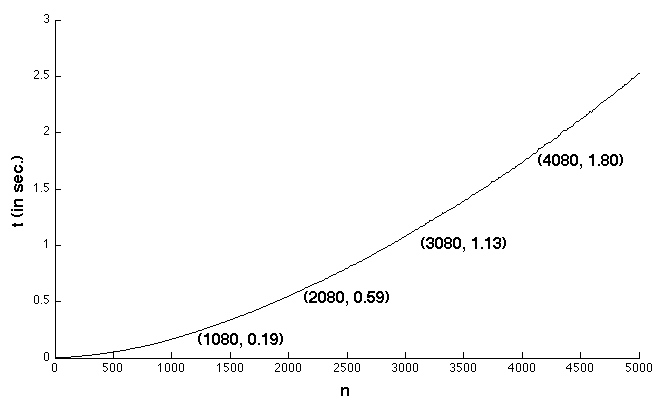
\includegraphics[scale=0.75]{complexity}
    %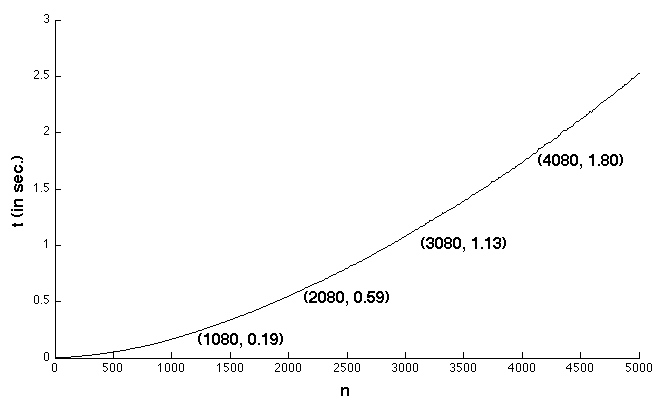
\includegraphics[]{complexity}
    %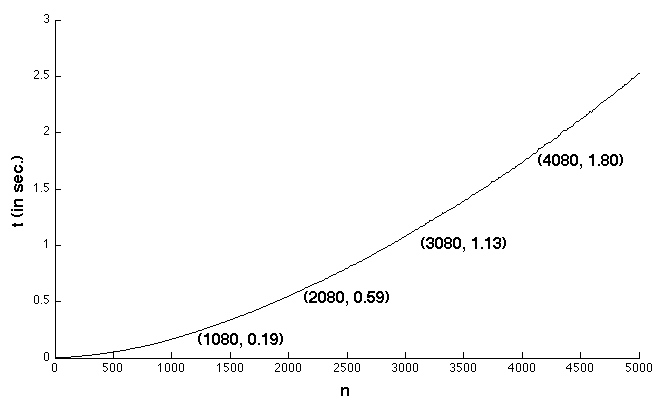
\includegraphics[width=0.9\linewidth,height=2.5in]{complexity}
    \caption{CAP time complexity versus no. of future observations.}
    \label{fig:complexity}
\end{figure}
\hspace{0.3cm}
\begin{figure}
    \centering
    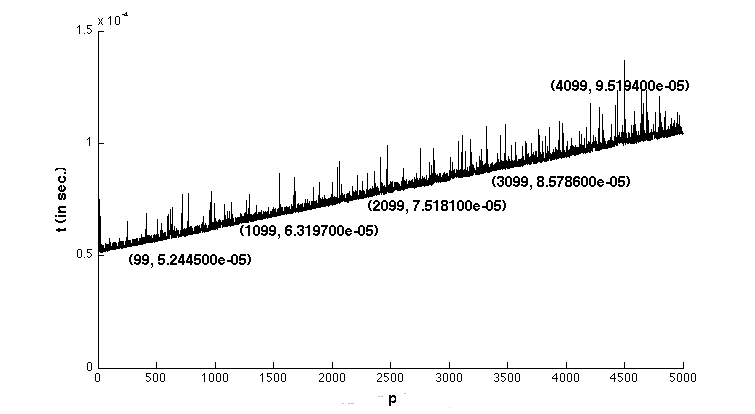
\includegraphics[scale=0.75]{complexity_p}
    %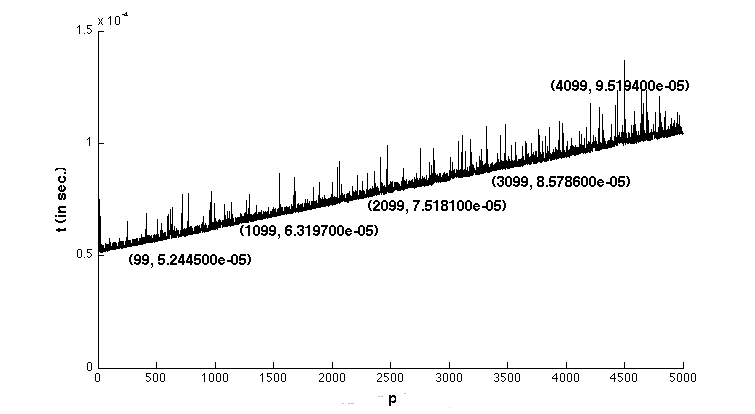
\includegraphics[width=1.0\linewidth,height=2.5in]{complexity_p}
    \caption{CAP time complexity versus no. of past observations.}
    \label{fig:complexityp}
\end{figure}

\section{Effective Thermal Prediction}
\label{sec:effect-therm-pred}
CAP is an estimator for the system level energy consumption as expressed
in \ref{eq:linmodel}.  In turn, the estimate can be combined with
temperature measurements, PeCs, and system metrics 
to create a Thermal Chaotic Attractor Predictor (TCAP). TCAPs
differ from CAPs by their nature as thread level rather than system
level predictors.  As such, we keep track on a per-thread basis of the
observables used in prediction.

\begin{table}[tbph]
  \centering
  \caption{Additional thermal benchmarks}
  \label{tab:thermalbench}
% BEGIN RECEIVE ORGTBL thermalbench
\begin{tabular}{lll}
\hline
\hline
hpl & C & Linear algebra \\
stream & C & Memory stress testing \\
aluadd & Assembly & Processor \\
therm & Assembly & Thermal stress test \\
\hline
\end{tabular}
% END RECEIVE ORGTBL thermalbench
\begin{comment}
#+ORGTBL: SEND thermalbench orgtbl-to-latex :splice nil :skip 0
|--------+----------+-----------------------|
|--------+----------+-----------------------|
| hpl    | C        | Linear algebra        |
| stream | C        | Memory stress testing |
| aluadd | Assembly | Processor             |
| therm  | Assembly | Thermal stress test   |
|--------+----------+-----------------------|
\end{comment}
\end{table}

We define a TCAP for each of the metrics in \equationname~\ref{eq:tea},
\equationname~\ref{eq:thermeff}, and \equationname~\ref{eq:thermcost}
using the procedure defined in Section~\ref{sec:cappcreate}.  For
thermal purposes, we construct the training set using the benchmarks in
\ref{tab:specbenchs} + the benchmarks listed in 
Table~\ref{tab:thermalbench}.  The additional benchmarks address the
issue in the training set of the behavior of the system under extreme
thermal stress. 

% Following comment block used by GNU-EMACS and AUCTEX packages
% Please do not remove.
%%% Local Variables: 
%%% mode: latex
%%% TeX-master: "prospectus.tex"
%%% End: 

% 
% File:     evaluation.tex
% Author:   awl8049
% Revision: 
% 
\chapter{Chaotic Attractor Predictor Evaluation}
\label{chp:evaluation}
Experiments were carried out to evaluate the performance of the CAP
power models built for approximating dynamic system solutions.  The
first experiment aimed to confirm the time complexity of CAP.  Making
use of MATLAB, our CAP code was executed on the two servers specified in
Table~\ref{tab:hardware}.  As the execution times on both servers
provide the same trend, only those collected from the SUN Fire 2200
server (AMD Opteron) are demonstrated here.  The code execution time
results versus $n$ (the number of future observations) is illustrated in
\figurename~\ref{fig:complexity}, where the result curve confirms CAP
time complexity in $O(n^{2})$.  Separately, the CAP execution time as a
function of $p$ (the number of past observations) on the SUN Fire server
is shown in \figurename~\ref{fig:complexityp}, where the time indeed is
linear with respect to $p$, as claimed earlier in our time complexity
subsection.  In practice, a moderate $p$ (of, say, 100) and a small $n$
(of, say, 5) may be chosen under CAP for high accuracy and very low time
complexity in real-time applications.  The results of distant future
(corresponding to a larger $n$) can be predicted by a step-wise process,
with each step predicting the near future outcomes (using $n$ = 5).

\begin{table}[t]
  \centering
  \caption{Server configurations for evaluation}
  \label{tab:hardware}
  \begin{tabular}{l l l}
   \hline
    &\textbf{Sun Fire 2200}&\textbf{Dell PowerEdge R610}\\  
    \hline
    CPU&2 AMD Opteron&2 Intel Xeon (Nehalem) 5500\\
    CPU L2 cache&2x2MB&4MB\\
    Memory&8GB&9GB\\
    Internal disk&2060GB&500GB\\
    Network&2x1000Mbps&1x1000Mbps\\
    Video&On-board&NVIDA Quadro FX4600\\
    Height&1 rack unit&1 rack unit\\
    \hline
  \end{tabular}
\end{table}

\begin{table}[t]
  \centering
  \caption{SPEC CPU2006 benchmarks used for evaluation}
  \label{tab:addspec}
  \begin{tabular}{c c p{5cm}}
    \hline
    \multicolumn{3}{l}{\textbf{Integer Benchmark}} \\
    \hline
    Astar&C++&Path Finding\\
    Gobmk&C&Artificial Intelligence: Go\\
    \multicolumn{3}{l}{\textbf{FP Benchmarks}} \\
    \hline
    Calculix&C++/F90&Structural Mechanics\\
    Zeusmp&F90&Computational Fluid Dynamics\\
    \hline
  \end{tabular}
\end{table}

\section{Evaluation environment}
\label{sec:measurementtools}
The operating system used in our test servers is OpenSolaris (namely,
Solaris 11).  Evaluation results are collected from the system baseboard
controller using the IPMI interface via the OpenSolaris
\texttt{ipmitool} utility.  Processor performance counters are collected
on a system-wide basis by means of \texttt{cpustat}, \texttt{iostat},
and \texttt{ipmitool} utilities in OpenSolaris.  Of these,
\texttt{iostat} and \texttt{ipmitool} are available across all
UNIX-based operating systems commonly employed by data centers, while
\texttt{cpustat} is an OpenSolaris-specific utility (which is being
ported to Linux).

\begin{table}[t]
  \centering
  \caption{Branch and Memory Access Patters of Evaluation Benchmarks}
  \label{tab:benchstats}
\begin{tabular}{lllllrrr}
\hline
% BEGIN RECEIVE ORGTBL perfmetrics
Benchmark & Inst Count & Branches & Loads & Stores \\
 & (Billions) &  &  &  \\
\hline
astar & 1,200 & 15.57\% & 40.34\% & 13.75\% \\
gobmk & 1,603 & 19.51\% & 29.72\% & 15.25\% \\
calculix & 3,041 & 4.11\% & 40.14\% & 9.95\% \\
zeusmp & 1,566 & 4.05\% & 36.22\% & 11.98\% \\
\hline
% END RECEIVE ORGTBL perfmetrics
\end{tabular}
\end{table}
\begin{comment}
#+ORGTBL: SEND perfmetrics orgtbl-to-latex :splice t :skip 0
| Benchmark | Inst Count | Branches | Loads   | Stores  |
|           | (Billions) |          |         |         |
|-----------+------------+----------+---------+---------|
| astar     | 1,200      | 15.57\%  | 40.34\% | 13.75\% |
| gobmk     | 1,603      | 19.51\%  | 29.72\% | 15.25\% |
| calculix  | 3,041      | 4.11\%   | 40.14\% | 9.95\%  |
| zeusmp    | 1,566      | 4.05\%   | 36.22\% | 11.98\% |
|-----------+------------+----------+---------+---------|
\end{comment}

Four benchmarks from the SPEC CPU2006 benchmark suite were used for the
evaluation purpose, as listed in Table~\ref{tab:addspec}), and they are
different from those employed earlier for CAP creation (as listed in
Table V). It is noted that selection of benchmarks for both calibration
and evaluation were selected to sufficiently exercise processor, cache,
and memory again per the decision criteria in \cite{Phansalkar2007},
with the additional criterion of selecting workloads more common to
server environments. As illustrated in Table~\ref{tab:benchstats}
(per results from \cite{Phansalkar2007}), the mix of instructions
exercises the key components of processor, memory, and cache in the
dynamic system which we model with CAP. In addition, the four
benchmarks used in our evaluation represent the type of high-utilization
workloads in server environments per typical industry use of the SPEC
CPU2006 benchmark suite \cite{Cisco2010}.
\begin{table}[]
  \caption{Model errors for CAP (under $n=5$, $p=100$, $r=14$), AR(1),
    MARS, and EWMA on AMD Opteron server}
  \centering
    \label{tab:modelerroropt}
    \begin{tabular}[phtb]{c | r r c | r r c}
      \hline
      \multicolumn{1}{c|}{}&\multicolumn{3}{c|}{\textbf{CAP}}&\multicolumn{3}{c}{\textbf{AR}}\\
      \hline
  &\multicolumn{1}{c}{\textbf{Avg}}&\multicolumn{1}{c}{\textbf{Max}}&\multicolumn{1}{c|}{\textbf{RMSE}}&\multicolumn{1}{c}{\textbf{Avg}}&\multicolumn{1}{c}{\textbf{Max}}&\multicolumn{1}{c}{\textbf{RMSE}}\\
\multicolumn{1}{c|}{\textbf{Benchmark}}&\multicolumn{1}{c}{\textbf{Err \%}}&\multicolumn{1}{c}{\textbf{Err \%}}&\multicolumn{1}{c|}{}&\multicolumn{1}{c}{\textbf{Err \%}}&\multicolumn{1}{c}{\textbf{Err \%}}&\multicolumn{1}{c }{\textbf{}}\\
        \hline
      Astar &0.9\%&5.5\%&0.72&3.1\%&8.9\%&2.26\\
      Games &1.0\%&6.8\%&2.06&2.2\%&9.3\%&2.06\\
      Gobmk &1.6\%&5.9\%&2.30&1.7\%&9.0\%&2.30\\
      Zeusmp&1.0\%&5.6\%&2.14&2.8\%&8.1\%&2.14\\
      \hline
      \multicolumn{1}{c|}{}&\multicolumn{3}{c|}{\textbf{MARS}}&\multicolumn{3}{c}{\textbf{EWMA}}\\
      \hline
  &\multicolumn{1}{c}{\textbf{Avg}}&\multicolumn{1}{c}{\textbf{Max}}&\multicolumn{1}{c|}{\textbf{RMSE}}&\multicolumn{1}{c}{\textbf{Avg}}&\multicolumn{1}{c}{\textbf{Max}}&\multicolumn{1}{c}{\textbf{RMSE}}\\
\multicolumn{1}{c|}{\textbf{Benchmark}}&\multicolumn{1}{c}{\textbf{Err \%}}&\multicolumn{1}{c}{\textbf{Err \%}}&\multicolumn{1}{c|}{}&\multicolumn{1}{c}{\textbf{Err \%}}&\multicolumn{1}{c}{\textbf{Err \%}}&\multicolumn{1}{c }{\textbf{}}\\
      \hline
      Astar &2.5\%&9.3\%&2.12&1.2\%&7.9\%&2.40\\
      Games &3.0\%&9.7\%&2.44&1.1\%&7.8\%&1.42\\
      Gobmk &3.0\%&9.1\%&2.36&1.0\%&6.9\%&2.30\\
      Zeusmp&2.8\%&7.9\%&2.34&1.8\%&9.2\%&2.01\\
      \hline
    \end{tabular}
  \end{table}

The benchmarks were executed on the two servers specified in
Table~\ref{tab:hardware}, with performance metrics gathered during the
course of execution.  Power consumed is measured by a WattsUP power meter
\cite{WattsUp2006a}, connected between the AC Main and the server under
test.  The power meter measures the total and average wattage,
voltage, and amperage over the run of a workload.  The internal memory
of the power meter is cleared at the start of each run and the measures
collected during the runs are downloaded (after execution completion)
from meter's internal memory into a spreadsheet.  Current flow on
different voltage domains in the server is measured using an Agilent
MSO6014A oscilloscope, with one Agilent 1146A current probe per server
power domain (12v, 5v, and 3.3v).  This data was collected from the
oscilloscope at the end of each benchmark execution on a server and then
stored in a spreadsheet on the test host.

\begin{figure}[]
  \centering
  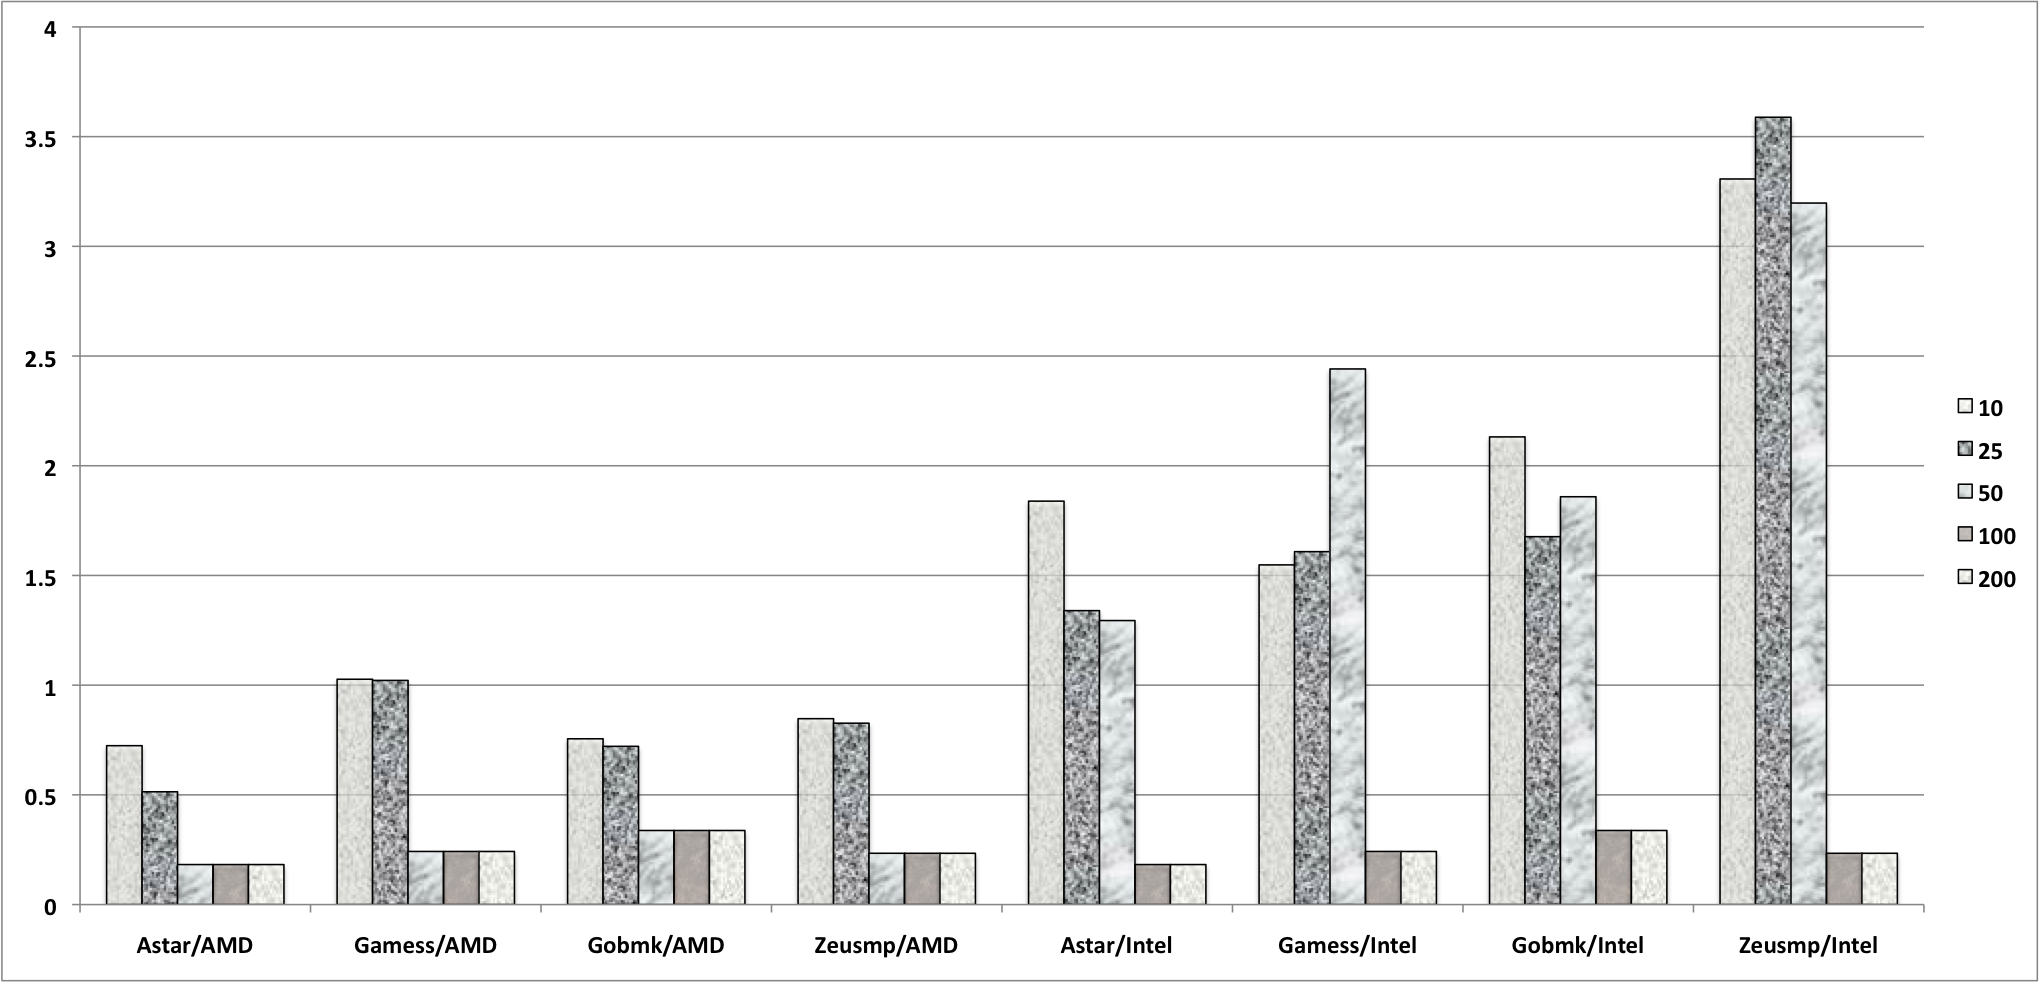
\includegraphics[width=1.0\linewidth,height=2.5in]{rmsep}
  \caption{Root Mean Square Error (RMSE) for different values of $p$.}
  \label{fig:rmsep}
\end{figure}
\section{Results}
\label{sec:htcase}
While the number of measures per observation ($r$) is fixed for a given
server in our evaluation (equal to 14 for the Sun Fire server and to 19
for Dell PowerEdge server), the CAP prediction time and accuracy depend
on $p$ (the number of past observations) and $n$ (the number of future
observations), as stated in Section~\ref{sec:cappcreate}.  In our
evaluation, the CAP prediction error rates of various benchmark codes
for a range of $p$ under a given $n$ were gathered, as demonstrated in
\figurename~\ref{fig:rmsep}, where $n$ equals 5.  It can be seen from
the figure that the error rates are fairly small (and stay almost
unchanged) when $p$ is within 100 to 200, but they rise considerably
when $p$ drops to 50 or below.  In subsequent figures, the prediction
results of CAP include only those for $n = 5$ and $p = 100$.  Each
benchmark was executed to collect the first $p=100$ points on the
attractor, at which point the next $n$=5 points were used to
compute the estimated power for the $t, t+1,\ldots,t+5$ energy estimates
in each time cycle.

\begin{figure}[]
  \centering
  \subfloat[Astar/CAP.]{%
    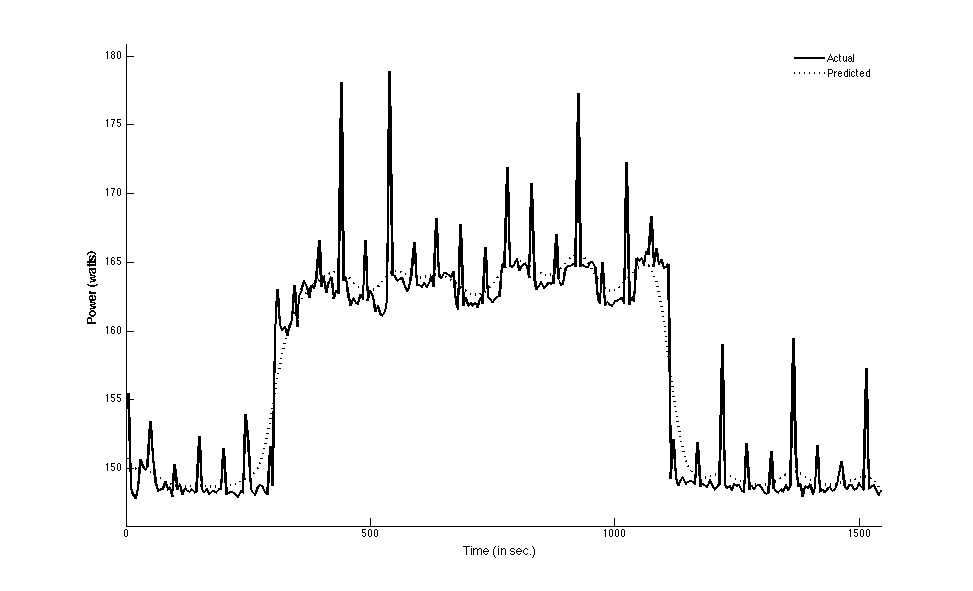
\includegraphics[width=0.5\linewidth,height=2in]{allpower/amd_ch_astar}
  }
  \subfloat[Astar/AR(1)).]{%
    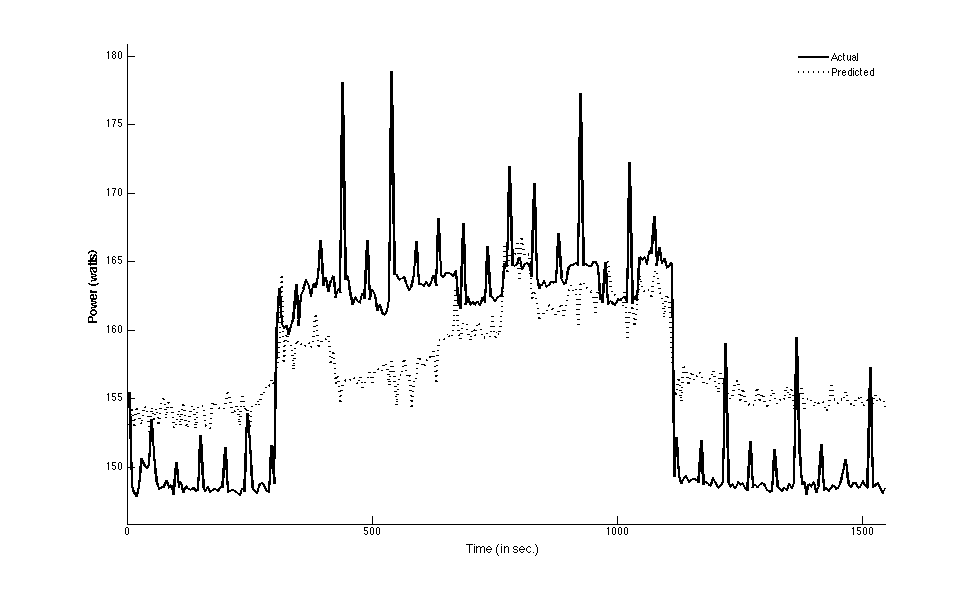
\includegraphics[width=0.5\linewidth,height=2in]{allpower/amd_ar_astar}
  }\\
  \subfloat[Zeusmp/CAP.]{%
    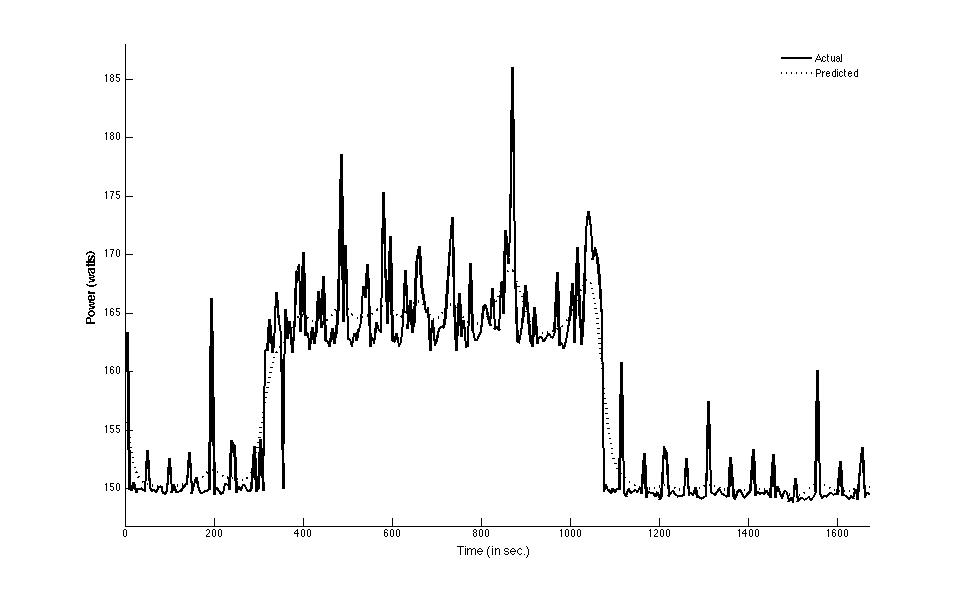
\includegraphics[width=0.5\linewidth,height=2in]{allpower/amd_ch_zeusmp}
  }
  \subfloat[Zeusmp/AR(1).]{%
    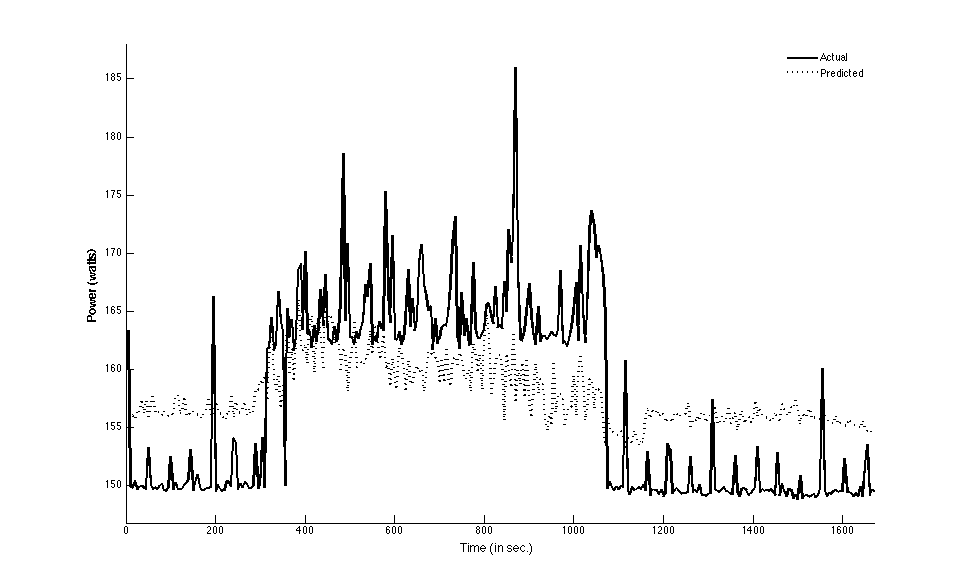
\includegraphics[width=0.5\linewidth,height=2in]{allpower/amd_ar_zeusmp}
  }
  \caption{Actual power results versus predicted results for AMD Opteron.}
  \label{fig:compareamd}
\end{figure}
The predicted power consumption results of CAP during the execution of
Astar and Zeusmp on a HyperTransport-based server are demonstrated in
\figurenames~\ref{fig:compareamd}(a) and \ref{fig:compareamd}(c).  The
predicted values are seen to track closely to the measured readings
(obtained using the WattsUP power meter and indicated by solid curves),
with the error rate ranging between 0.9\% and 1.6\%.  For comparison,
the predicted power consumption outcomes during the execution of same
selected benchmarks under AR(1) are depicted in
\figurenames~\ref{fig:compareamd}(b) and \ref{fig:compareamd}(d).  As
expected, AR(1) exhibits poor outcomes over any given short execution
window, with maximum errors ranging from 7.9\% to 9.3\%, despite that
the prediction error over the whole execution period may be less.  CAP
enjoys much better prediction behavior than its linear regressive
counterpart.

\begin{figure}[]
  \centering
  \subfloat[Astar/CAP.]{%
    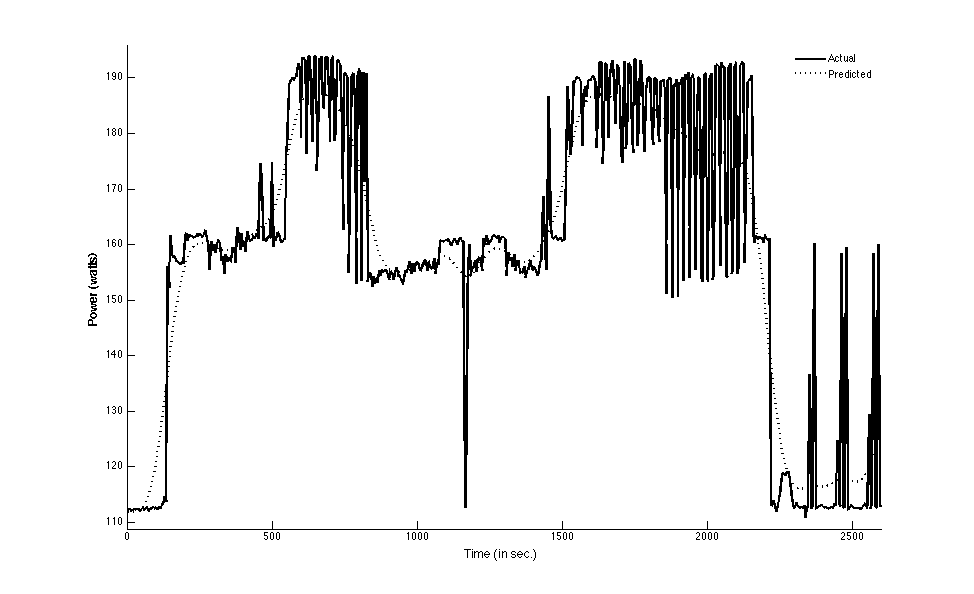
\includegraphics[width=0.5\linewidth,height=2in]{allpower/intel_ch_astar}
  }
  \subfloat[Astar/AR(1)).]{%
    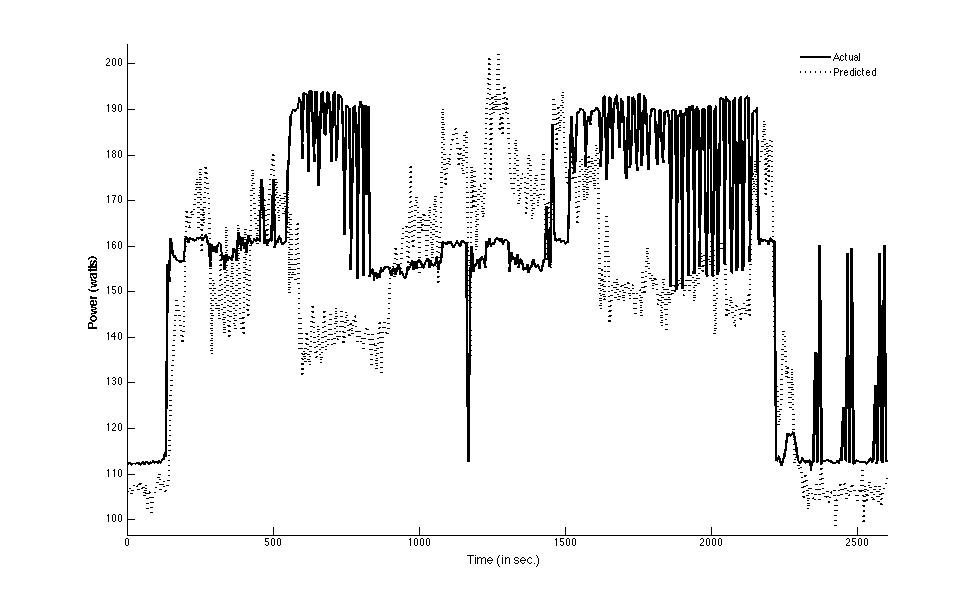
\includegraphics[width=0.5\linewidth,height=2in]{allpower/intel_ar_astar}
  }\\
  \subfloat[Zeusmp/CAP.]{%
    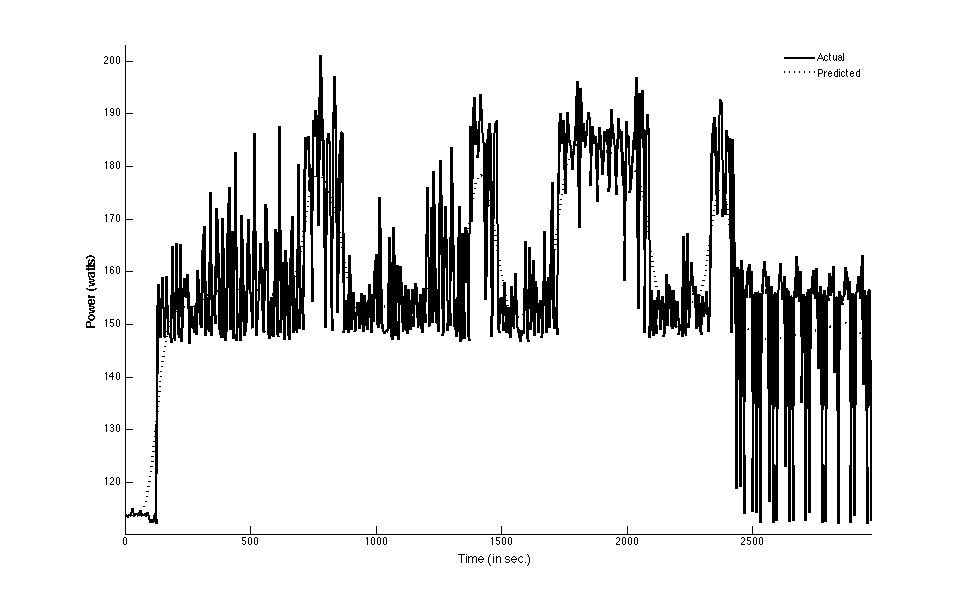
\includegraphics[width=0.5\linewidth,height=2in]{allpower/intel_ch_zeusmp}
  }
  \subfloat[Zeusmp/AR(1).]{%
    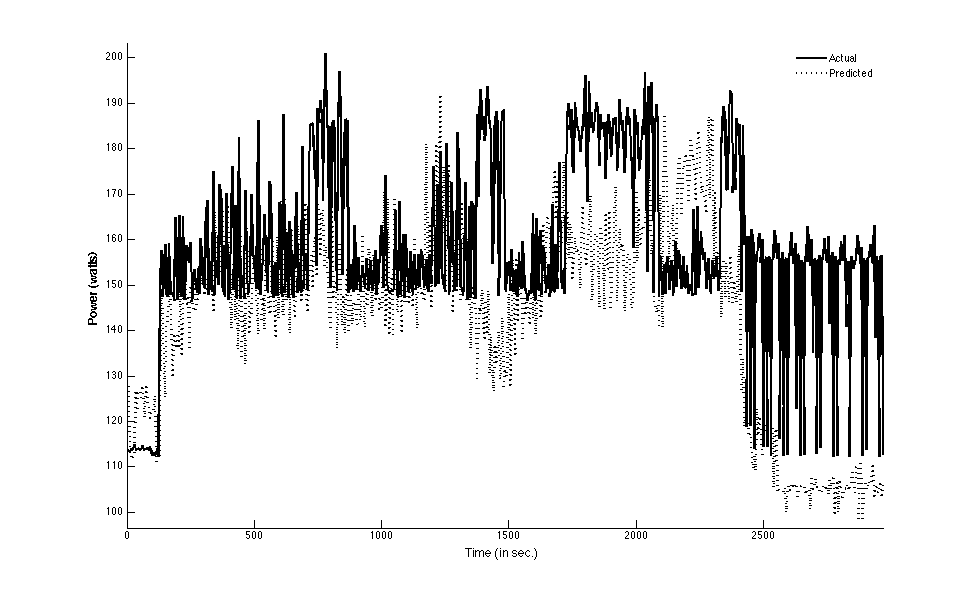
\includegraphics[width=0.5\linewidth,height=2in]{allpower/intel_ar_zeusmp}
  }
  \caption{Actual power results versus predicted results for an Intel
    Nehalem server.}
  \label{fig:compareintel}
\end{figure}
The predicted power consumption results under CAP over the benchmark
execution period for the QPL-based server (Dell PowerEdge) are
demonstrated in \figurenames~\ref{fig:compareintel}(a) and
\ref{fig:compareintel}(c), where the actual power consumption amounts
obtained by the WattsUP meter are shown by solid curves.  Again, CAP is
seen to exhibit impressive performance, tracking the actual amounts
closely, with the error rate ranging between 1.0\% and 3.3\%.  The root
mean square errors for CAP remain within small values.  In contrast,
AR(1) suffers from poor prediction behavior, as can be discovered in
\figurenames~\ref{fig:compareintel}(b) and \ref{fig:compareintel}(d),
where outcomes of same benchmarks executed on the Dell PowerEdge server
are depicted.  It yields the maximum error up to 20.8\% (or 20.6\%) for
the Astar (or Zeusmp) benchmark.  {\addtolength{\tabcolsep}{-3pt}
\begin{table}[]
  \footnotesize
  \caption{Model errors for CAP (under $n=5$, $p=100$, $r=19$), AR, MARS, and
    EWMA predictors on Intel Nehalem server}
  \centering
    \label{tab:modelerroroptIntel}
    \begin{tabular}[phtb]{c | r r c | r r c}
      \hline
      \multicolumn{1}{c|}{}&\multicolumn{3}{c|}{\textbf{CAP}}&\multicolumn{3}{c}{\textbf{AR}}\\
        \hline
  &\multicolumn{1}{c}{\textbf{Avg}}&\multicolumn{1}{c}{\textbf{Max}}&\multicolumn{1}{c|}{\textbf{RMSE}}&\multicolumn{1}{c}{\textbf{Avg}}&\multicolumn{1}{c}{\textbf{Max}}&\multicolumn{1}{c}{\textbf{RMSE}}\\
\multicolumn{1}{c|}{\textbf{Benchmark}}&\multicolumn{1}{c}{\textbf{Err \%}}&\multicolumn{1}{c}{\textbf{Err \%}}&\multicolumn{1}{c|}{}&\multicolumn{1}{c}{\textbf{Err \%}}&\multicolumn{1}{c}{\textbf{Err \%}}&\multicolumn{1}{c }{\textbf{}}\\
      \hline
      Astar &1.1\%&20.8\%&1.83&5.9\%&28.5\%&4.94\\
      Games &1.0\%&14.8\%&1.54&5.6\%&44.3\%&5.54\\
      Gobmk &1.0\%&21.5\%&2.13&5.3\%&27.8\%&4.83\\
      Zeusmp&3.3\%&20.6\%&3.31&7.7\%&31.8\%&7.24\\
      \hline
      \multicolumn{1}{c|}{}&\multicolumn{3}{c|}{\textbf{MARS}}&\multicolumn{3}{c}{\textbf{EWMA}}\\
      \hline
  &\multicolumn{1}{c}{\textbf{Avg}}&\multicolumn{1}{c}{\textbf{Max}}&\multicolumn{1}{c|}{\textbf{RMSE}}&\multicolumn{1}{c}{\textbf{Avg}}&\multicolumn{1}{c}{\textbf{Max}}&\multicolumn{1}{c}{\textbf{RMSE}}\\
\multicolumn{1}{c|}{\textbf{Benchmark}}&\multicolumn{1}{c}{\textbf{Err \%}}&\multicolumn{1}{c}{\textbf{Err \%}}&\multicolumn{1}{c|}{}&\multicolumn{1}{c}{\textbf{Err \%}}&\multicolumn{1}{c}{\textbf{Err \%}}&\multicolumn{1}{c }{\textbf{}}\\
      \hline
      Astar &5.4\%&28.0\%&4.97&3.7\%&32.4\%&2.98\\
      Games &4.7\%&33.0\%&4.58&1.8\%&27.3\%&2.19\\
      Gobmk &4.1\%&27.9\%&4.73&3.9\%&28.4\%&2.73\\
      Zeusmp&11.6\%&32.2\%&8.91&5.0\%&31.3\%&2.81\\
      \hline
    \end{tabular}
  \end{table}
}
\section{Further discussion}
\label{sec:caseanalysis}
Tables~\ref{tab:modelerroropt} (or \ref{tab:modelerroroptIntel})
compares the errors of evaluation benchmarks for the server with the
HyperTransport (or QPL) structure, under four different prediction
mechanisms: CAP, AR, MARS, and EWMA. Large errors exhibited by AR,
MARS, and EWMA overwhelm the advantages gained from their simplicity.
The table results indicate the limitations entailed by using a linear
technique, such as AR time series, to predict dynamic system behavior;
similar issues exist for piecewise and moving average techniques, such as
MARS and EWMA.  Earlier attempts were made to address this issue by
incorporating corrective mechanisms in combination with these
predictors.  An example attempt employed machine learning to monitor 
mis-prediction, with recalibration invoked when required
\cite{Coskun2008}.  CAP eliminates the need for any corrective mechanism
by directly addressing the system dynamics, thereby avoiding wide drifts in
prediction experienced by other prediction techniques.

The model developed in this work is valid for any
dual-core/dual-processor system using NUMA memory access connected in a
point-to-point manner using the HyperTransport or the QPL structures.
However, it can be scaled to quad-core dual processors based on those
two structures.  One would expect to see a slight difference or
variation in power prediction due to a greater or less affect of die
temperatures on the other performance measures.  Under a dual-core
quad-processor server, for example, additional regression variables
would be incorporated in $E_{proc}$, giving rise to more performance
measures (i.e., a larger $r$).  Similarly, more PeCs related to cache
misses would then be involved in $E_{mem}$.  The solution approach of
CAP remains exactly identical, except for a larger $r$ in its prediction
computation.

% Following comment block used by GNU-EMACS and AUCTEX packages
% Please do not remove.
%%% Local Variables: 
%%% mode: latex
%%% TeX-master: "dissertation.tex"
%%% TeX-PDF-mode: t
%%% TeX-source-correlate-mode: t
%%% End: 

%
% File:     chapter-schedule.tex
% Author:   awl8049
% Revision: $Revision: 1.2 $
%
\chapter{Thermal-Aware Scheduling}
\label{chp:schedule}
The current generation of operating systems treat the cores in a
multicore processor as distinct physical processors. Furthermore, the
advent of simultaneous multi-threading (such as Intel's HyperThreading
technology) has led to operating systems treating such virtualized
processors as equal ``logical CPUs'' that behave as independent
processors for scheduling purposes.  However, there are dependencies
between these logical CPUs that need to be taken into account when
balancing performance and energy efficiency.  These dependencies lead to
contention for shared resources which, in turn, leads to performance
penalties and inefficient use of energy.  The component of the operating
system most aware of the existence of multiple cores is the thread
scheduling algorithm.  The scheduler is responsible for ensuring that
all of the cores across all processors in a system is kept busy; the
scheduler must be able to efficiently migrate the state of threads
across processors regardless if that migration remains on a core or
across processors.

Modern multiprocessor operating systems such as Windows, Linux, Solaris,
and FreeBSD take a two-level approach to scheduling in an attempt to
maximize system resources.  The first level manages each core using a
distributed run queue model with per core queues and fair scheduling
policies. The second level attempts to balance the resource load by
redistributing tasks across the queues on each core.  The design of such
schedulers are based upon three principles: (1) threads are assumed to
be independent, (2) load is equated to queue length, and (3) locality is
important \cite{Hofmeyr2010}.

Traditional server load balancing makes assumptions about workload
behavior to make scheduling decisions.  Interactive workloads are
characterized by the independent tasks that remain quiet for extended
periods.  Server workloads contain large numbers of threads that are
highly independent of each other that use synchronization objects to
ensure mutual exclusion on small data items.  In parallel applications,
there is a higher levels of interaction between threads; consequently,
load balancing such applications requires additional mechanisms.  

Parallel applications are implemented most often on contemporary
processors using a Single Process, Multiple Data (SPMD) programming
model where logical CPUs simultaneously execute the same program at
independent points.  Tasks execute independently and communicate with
other nodes by sending and receiving messages with some form of barrier
synchronization implemented as part of the message interface.  The
details of the message process is isolated from the application by
standard interfaces such as MPI and OpenMP. %need cites!
Note how this programming model contravenes the assumptions for system
level load balancing: (1) threads are logically related, (2) have data
and control dependencies between threads, and (3) have equally long
life-spans \cite{Hofmeyr2010}.  

Our scheduler extends the existing dispatcher and power
management infrastructure in the operating system. It is the role of the
kernel thread scheduler to manage the placement of threads in a dispatch
queue, decide which thread to run on a processor, and manage the
movement of threads to and from processors so as to balance the workload
amongst logical CPUS.  A scheduler must fulfill this role while
addressing two major requirements for SPMD applications: (1) threads
composing an application must make equal progress and (2) the maximum
level of hardware parallelism is exploited.

However, these schemes do not take into account the increase in thermal
stress placed upon the processor entailed by focusing on maximum
performance.  Modern processors crudely manage this problem through Dynamic
Thermal Management (DTM) where the processor monitors the die
temperature and dynamically adjusts the processor voltage and frequency
(DVFS) to slow down the processor.  Prior work
\cite{Bircher2008,Donald2006,Coskun2008d} has shown that this technique has
significant negative impact on both performance and reliability in the
processor.   Thus, pro-active scheduling techniques that avoid thermal
emergencies are preferable to reactive hardware techniques such as DTM.

\section{Thread Selection}
\label{sec:whatnext}
The scheduler is responsible in each quantum for deciding which thread
to run on a processor.  We introduce in this work a heuristic scheduling
algorithm that reduces the thermal stress on a multicore processor
while addressing the SPMD requirements of equal progress and maximum
exploitation of parallelism.  The thermal predictor introduced in
Chapter~\ref{sec:themalmodel} is used to construct a on-line thermal
estimator for temperature, which is then used to predict which thread to
next execute on each logical CPU's run queue.

We enhance the existing thread infrastructure to maintain
the information required by the thermal estimator. Our implementation is
based upon the concept of Task Activity Vectors (TAVs) as introduced by 
\citeN{Merkel2008a}.  Each task maintains a vector with the required
history needed to make a prediction; in effect, we trade the additional
space required for keeping this history for the benefits gained from the
thermal scheduling.   At each scheduling quantum, each TAV is updated
with counts from the performance counters representing the hardware
resources used in the predictor.   The scheduler predicts the impact on
the logical CPU temperature using the thermal predictor to map the
PeCs values into an estimate of the ``thermal efficiency of
application'' (TEA) (as discussed in \ref{sec:themalmodel}).  

The predictions are then used by a policy-based heuristic predictor to
decide which thread to execute given the TEA of each candidate thread.
The operating system kernel is enhanced to allow the policy to be
selected as a kernel configuration option. We examine the behavior of
our predictor against three well known thermal scheduling heuristics:
(1) Greedy, (2) MinTemp \cite{Kursun2006}, and (3) ThreshHot
\cite{Zhou2010b}.  The Greedy heuristic selects the coolest job to
execute in each scheduling epoch, MinTemp selects the coolest possible
thread if over a set threshold, and ThreshHot selects the hottest thread
that is predicted to not cause the temperature to exceed that set
threshold or the hottest job in the queue otherwise.

\section{Load Balancing}
\label{sec:loadbalance}
Load balancing distributes workload evenly across the available logical
CPUs; current implementations distribute to maximize performance, we
enhance the concept to minimize thermal stress while seeking best
performance. We begin by organizing the logical CPUs in the system into
three categories based upon the temperature at which a DTM event occurs:
Hot (90\% of DTM temperature), warm (between 75\% and 90\% of DTM
temperature), and cold (less than 75\% of the DTM temperature).  In
addition, we classify each logical CPU into ``clans'' depending whether
a logical CPU is considered a ``fast processor'' or ``slow processor''
depending upon the current processor frequency of the underlying
hardware.  This two-level categorization allows us to manage the
distribution of work such that we can migrate work away from heat
sources while minimizing the impact on performance of threads.

The movement of logical CPUs between processor groups as temperature
increases is managed by a Thermal Predictor.  The Thermal Predictor
collect the values of the PeCs, temperature readings from the logical
CPUS, and utilization data from the dispatcher to decide whether a
processor will move towards the DTM temperature.  In this way we can
anticipate the DTM event and prevent its occurrence.

\begin{figure}[htbp]
  \centering
  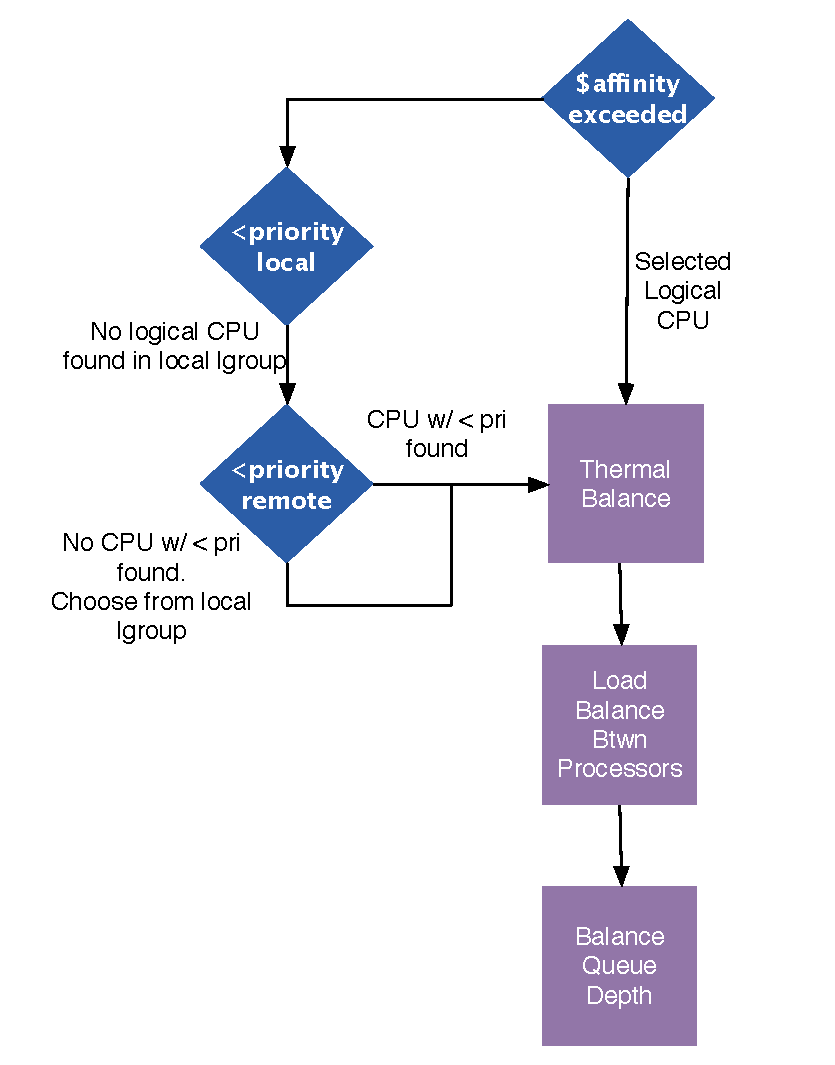
\includegraphics[scale=0.40]{threadinsert.pdf}
  \caption{Thread Queue Insertion}
  \label{fig:thread}
\end{figure}
The dispatcher is responsible for deciding where to insert threads into
run queues; i.e., when and where a thread will next execute. The steps
in this process are illustrated in Figure~\ref{fig:thread}.  First, the
dispatcher checks to see if the logical CPU where the thread was running
satisfies the cache affinity criteria (the default for OpenSolaris is
the thread was last running within the past 3 cycles).  If that test
fails, it tries to find the logical CPU in the local group running the
lowest priority thread.  If no thread is found in the local group, then
the dispatcher will check through known remote groups.  If no logical
CPU is found in either case, it will choose a logical CPU in the local
group.

At this point, the system will attempt to load balance the workload.
Two possibilities exist in the current system: equal balance across all
physical processors in the system and coalesce work onto one chip or the
other.  The first case is traditional example of load balancing while
the second case is attempting to free up as many resources as possible
to provide opportunities for power management to find logical units to
shut down.  We add a third sort of load balancing: temperature
balance. In this case, the dispatcher will attempt to load logical CPUs
in the ``COLD'' processor group first, followed by the ``WARM''
processor group, and finally the ``HOT'' group.

\subsection{Algorithm}
\label{sec:lbalgorithm}
Our Thermal-Aware Balancer (TAB) uses two classes of threads: a global
Thermal Predictor Thread (TPT) and multiple Thermal Balancing Threads
(TBT), one TBT per logical CPU.   The Thermal Predictor Thread is a
temperature monitor that watches the temperature of the logical CPU and
adjusts the HOT, WARM, COLD lists on a periodic basis.  The TBTs on each
logical CPU performs a mix of speed and thermal balancing
\cite{Hofmeyr2010} on queues assigned to each logical CPU.

The TPT awakes periodically and enumerates the known logical CPUs to
rearrange the HOT, WARM, COLD list.   The uses the thermal predictor
defined in the previous chapter to evaluate the past behavior of each
logical CPU and adds/deletes this unit from the appropriate
lists. 

\begin{lstlisting}[float,label=code:TABbalance,caption=TAB Balancing Algorithm]
begin
Determine if logical CPU is HOT, WARM, or COLD
if logical cpu is HOT
begin
   for each thread in the run queue
     begin
         Project the resulting change in temperature if this thread
         executes
         Compute the projected logical CPU speed over the elapsed balance
         interval
     end
   Compute the global core speed as average over all logical CPUs
   Migrate the thread with the ``worst'' impact on temperature to the
   logical CPU in the COLD set most suitable from a speed standpoint.
end
\end{lstlisting}
Periodically, the TBT on each core wakes up, check for imbalances
on the on the core and pulls threads from the hotter cores to local
cores and return to sleep.    Note that this is a distributed algorithm
where each TBT operates independently and without any global
synchronization.   A TBT executes the code in
Listing~\ref{code:TABbalance} when it awakes in order to adjust the
thermal balance of the queues in the designated logical CPU.


% Following comment block used by GNU-EMACS and AUCTEX packages
% Please do not remove.
%%% Local Variables: 
%%% mode: latex
%%% TeX-master: "prospectus.tex"
%%% End: 

%
% File:     chapter-scheduler-evaluation.tex
% Author:   awl8049
% Revision: $Revision: 2.1 $
\chapter{Thermal Aware Scheduler Evaluation}
\label{chp:scheduler-evaluation}
We have evaluated our TAS (Thermal Aware Scheduler) using the FreeBSD
operating system run on a commodity server.  Our TAS implementation
modified the existing push migration in FreeBSD's ULE
scheduler~\cite{Roberson2003,McKusick2004,McKusick2004b} to take into
account both thermal behavior and system performance, as elaborated in
Chapter~\ref{chp:schedule}.  PeC data were collected at the user level
through standard tools provided for the data collection purpose by
FreeBSD (i.e., the \texttt{coretemp} and \texttt{hwpmc} kernel
extensions).  They were collected and collated by a FreeBSD kernel
extension, made available to the operating system scheduler for query
when making scheduling decisions (\figurename~\ref{fig:teaplant})

The processor thermal model was calibrated by measuring behavior
outcomes of the testbed with TAS at idle and under high load stress
using common utilities from the FreeBSD regression test suites and
software collections.  The CPU-related behavior of our scheduler was
then characterized using integer and floating point benchmarks from the
SPEC CPU2006~\cite{Henning2006} benchmark suite.  Benchmarks from the
Princeton Application Repository for Shared-Memory Computers (PARSEC)
suite~\cite{Bienia2008} were then evaluated on the testbed to assess TAS
in terms of key metrics of interest (i.e., die temperature and benchmark
run time) under high parallelism in the thread level.

\begin{table}[tbhp] 
\centering
  \caption{Processor used in evaluation}
  \label{tab:hardware}
  \begin{tabular}{l l} 
\hline 
\hline
&\textbf{Dell Precision 490}\\ 
\hline 
CPU&Intel Xeon 5300 (Woodcrest)\\ 
CPU L2 cache&4MB\\ 
Memory&8GB, DDR2 667Mhz with ECC\\
Internal disk&500GB\\ 
Network&1x1000Mbps\\ 
Video&NVIDA Quadro FX3400\\ 
\hline
  \end{tabular}
\end{table}
\section{Experiment Setup}
\label{sec:experiment-setup} 
Experimental evaluation was conducted on our testbed running TAS, with
its hardware specified in Table~\ref{tab:hardware}.  The key metrics of
interest were gathered during the course of application execution.
Power consumed was measured by a WattsUP power meter
\cite{WattsUp2006a}, connected between the AC Main and the server
testbed.  The power meter measured the total and average wattage,
voltage, and amperage over the run of a workload.  The internal memory
of the power meter was cleared at the start of each run and the measures
collected during the runs were downloaded (after execution completion)
from the meter's internal memory into a spreadsheet.

\section{SPEC Benchmark Results and Discussion}
\label{sec:microarch} 
Benchmarks from the SPEC CPU2006 suite \cite{Henning2006} were used to
evaluate the thermal behavior of CPU-bound workloads executed on our
testbed with the TAS scheduler.  The benchmarks were selected to
represent real life applications under various levels of thermal
stress. It has been shown previously \cite{Choi2007,Cher2011} that
significant core-to-core and functional unit-to-functional unit thermal
variations occur on modern processors, with the result that different
workload characteristics have strong influence on the power and thermal
behavior of the processor~\cite{Jimenez2010}.  We thus consider mixing
integer and floating-point SPEC CPU2006 benchmarks for concurrent
execution on the four cores of our testbed processor.  

\begin{table}[t]
  \centering
  \caption{Branch and Memory Access Patters of Evaluation Benchmarks}
  \label{tab:mixstats}
\begin{tabular}{lrrrrr}
\hline
\multicolumn{1}{l}{\textbf{Benchmark}}& \multicolumn{1}{c}{\textbf{Inst Count}} & \multicolumn{1}{c}{\textbf{Branches}}&\multicolumn{1}{c}{\textbf{Loads}} & \multicolumn{1}{c}{\textbf{Stores}} \\
 & \multicolumn{1}{c}{\textbf{(Billions)}}&  &  &  \\
\hline
namd & 2.483 & 4.28\% & 35.45\% & 8.83\% \\
hmmer & 3,363 & 7.08\% & 47.36\% & 17.68\% \\
mcf & 327 & 21.17\% & 37.99\% & 10.55\% \\
milc & 937 & 1.51\% & 40.15\% & 12.98\% \\
\hline
\end{tabular}
\end{table}
Three workload mixes are considered, and they span a range of cases,
including high-IPC/low-IPC, hot/cold thermal profiles \cite{Kursun2008},
and integer/floating-point combinations~\cite{Phansalkar2007} for better
evaluating our scheduler under diverse workload variations.  As
illustrated in Table~\ref{tab:mixstats}, the mix of instructions in the
selected benchmarks benchmark exercises the key components of the
processor, memory, and cache to create workloads with varying levels of
thermal stress. The three workload mixes are as follows: Workload Mix
$A$ = \{\texttt{namd}, \texttt{namd}, \texttt{hmmer}, \texttt{mcf}\},
Workload Mix $B$ = \{\texttt{milc}, \texttt{milc}, \texttt{namd},
\texttt{hmmer}\} and Workload Mix $C$ = \{\texttt{milc}, \texttt{mcf},
\texttt{mcf}, \texttt{hmmer}\}.  For example, Workload Mix $B$ involved
three copies of floating-point benchmarks (i.e., \texttt{milc},
\texttt{milc}, and \texttt{namd}) and one integer benchmark,
\texttt{hmmer}.  The memory intensive benchmarks (for instance, the
\texttt{milc} benchmark) tend to consume more power when executed as
opposed to other benchmarks in the suite while benchmarks with higher
IPC (the \texttt{mcf} and \texttt{hmmer} benchmarks) tends to increase
core on-die temperatures.

\begin{table}[tbp] 
\centering
\caption{Temperature and runtime results under benchmark mixes}
\label{tab:mixwkload}
\begin{tabular}{cllllll} 
\hline
\hline
\textbf{Workload} & \multicolumn{4}{c}{\textbf{Core die temperature reduction}} & \textbf{Runtime}\\
 \textbf{Mix} & \textbf{Core 0} & \textbf{Core 1} & \textbf{Core 2}  & \textbf{Core 3} & \textbf{increase} \\
\hline
$A$ & 2.8$^{\circ}$C & 1.0$^{\circ}$C & 1.7$^{\circ}$C & 2.0$^{\circ}$C & 2.1\% \\
$B$ & 1.0$^{\circ}$C & 0.8$^{\circ}$C & 2.0$^{\circ}$C & 1.1$^{\circ}$C & 2.9\% \\
$C$ & 3.1$^{\circ}$C & 3.3$^{\circ}$C & 3.0$^{\circ}$C & 2.9$^{\circ}$C & 2.5\% \\
\hline
\end{tabular}
\end{table}

It was observed that as execution progressed, the threads of those
benchmarks again tended to pin themselves to particular cores, depending
upon cache and memory utilization of other concurrent threads.  Core
temperatures are reduced under TAS in comparison to those under ULE,
with the reduction amounts listed in Table~\ref{tab:mixwkload} for the
three workload mixes.  Under Workload Mix $C$, for example, TAS lowers
core temperatures by at least 2.9$^{\circ}$C and by as much as
3.3$^{\circ}$C.  The benchmark run times (which reflect performance
degradation) increase negligibly always, ranging from 2.1\% to 2.9\%.

Involving both thermal-aware scheduling and load balancing, TAS compares
favorably with earlier workload migration-oriented methods, with
comparable reductions in average core die temperatures and performance
impact for similar workloads and processors.  Specifically,
Variation-Aware Core Hopping~\cite{Kursun2009} examined both thread
migration, by using off-line profiling of processor thermal variation to
guide assignment of threads to cores, and thread selection, by using the
profiling information to guide scheduling decisions in an enhanced Linux
scheduler.  This technique was demonstrated to lower core temperatures
ranging from 2.0$^{\circ}$C to 5.5$^{\circ}$C with pairs of SPEC CPU2006
benchmarks executed an IBM POWER5 processor with minimal overhead in the
decision process. However, their implementation did not performance
impact of logical cores sharing resources and the related
migration costs entailed by not considering cache affinity in scheduling
decisions.  Meanwhile, Predict-and-Act~\cite{Ayoub2011}
employs a hybrid reactive/proactive migration policy that controls
system fan speeds while scheduling threads at the core level.  This
hybrid method  was shown
to reduce on-die core temperatures by 3$^{\circ}$C to 4$^{\circ}$C on a
"simulated" pair of quad-core Intel Xeon processors (rather than a real
implementation) when executing mixes of SPEC2006 benchmarks similar to
those in our study.

\begin{table}[tbp] 
\centering
 \caption{PARSEC benchmarks used in evaluation}
\label{tab:parsecbench}
\begin{tabular}[bthp]{l l p{5cm}} 
\hline 
\hline 
bodytrack &  & Computer vision image tracking application \\
canneal &  & Simulated annealing chip routing cost computation \\
facesim &  & Physical simulation of facial behavior \\
ferret &  & Content-based similarity search \\
freqmine &  & Simulate FP-growth method for Frequent Itemset Mining \\
streamcluster &  & Online clustering algorithm for data mining \\
swaptions &  & Simulated pricing of portfolio options \\
\hline
\end{tabular}
\end{table}
\section{PARSEC Benchmark Results and Discussion}
\label{sec:mult-behav} 
Selected benchmarks from the PARSEC~\cite{Bienia2008} suite, described
in Table~\ref{tab:parsecbench}, were used to evaluate our TAS as well.
They were compiled with the POSIX \texttt{pthreads} library and executed
using the PARSEC \texttt{native} input sets.  Being parallel workloads
selected from the fields of computer vision, computational finance,
enterprise servers, and animation physics (see Table~\ref{tab:parsecbench}), PARSEC
benchmarks better represent real life applications than SPEC CPU2006 and
can benefit markedly from scheduling their abundant independent threads
freely based on thermal prediction.

\begin{figure}[tbp] 
\centering
  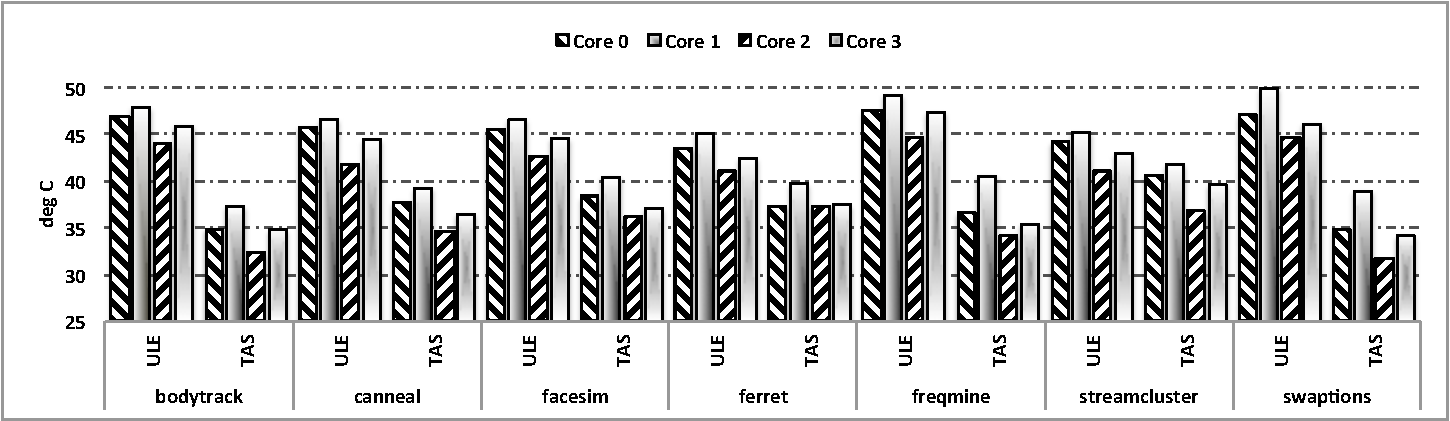
\includegraphics[width=1.0\linewidth,height=2.5in]{parsectemp}
  \caption{Comparison of PARSEC benchmark average core die temperatures
under ULE and TAS schedulers.}
  \label{fig:pbenchmarkt}
\end{figure}
Three behavior metrics of interest under TAS are gathered: (1) the
average core on-die temperature, (2) the benchmark run time, and (3)
mean system power dissipation.  The outcomes of average core on-die
temperatures upon executing those seven PARSEC benchmarks are depicted
in \figurename~\ref{fig:pbenchmarkt}.  As can be seen from the figure,
the core on-die temperatures range from 32$^\circ$C (for Benchmark
\texttt{swaption}) to 42$^\circ$C (for Benchmark \texttt{streamcluster})
under TAS, with \texttt{swaption} and \texttt{bodytrack} (or
\texttt{streamcluster}) experiencing the lowest (or highest) mean
temperature across the four cores.  Temperature outcomes for the same
benchmarks under the classical ULE scheduler are also included in
\figurename~\ref{fig:pbenchmarkt} for comparison.  It is found that
temperature reduction amounts are larger for benchmarks with smaller
working sets (like \texttt{bodytrack} and \texttt{swaptions}).  This is
because such a benchmark has a lower cache requirement \cite{Bienia2011}
and thereby lets TAS schedule threads more freely according to thermal
prediction with negligible performance degradation, resulting in better
temperature reduction.  Consequently, TAS enjoys temperature reduction
by more than 12.8$^{\circ}$C (from 44.8$^{\circ}$C down to
32.2$^{\circ}$C) for the \texttt{swaptions} benchmark.
  
Benchmarks with streaming functions, such as \texttt{facesim},
\texttt{freqmine}, and \texttt{streamcluster}, all have large working
sets, which hinder TAS from scheduling threads freely based on thermal
prediction, since doing so degrades performance considerably.  Hence,
those benchmarks tend to yield less temperature reduction under TAS,
with the average core on-die temperature lowered by 3-6$^{\circ}$C.  

Execution performance (measured in terms of the benchmark runtime) under TAS 
is depicted in \figurename~\ref{fig:pbenchmarkp}.
When compared with the runtime results under ULE included in the figure,
it can be observed that TAS leads to negligible performance degradation,
by no more than 3.3\% for all benchmarks examined except \texttt{streamcluster}.
Considerable performance degradation is seen for Benchmark \texttt{streamcluster},
however, likely due to its high computational intensity as the data set
grows with rising dimensionality and thereby calling for
more synchronization required.
As a result, TAS experiences noticeable performance degradation
when scheduling threads based on thermal prediction.

\begin{figure}[tbp]
  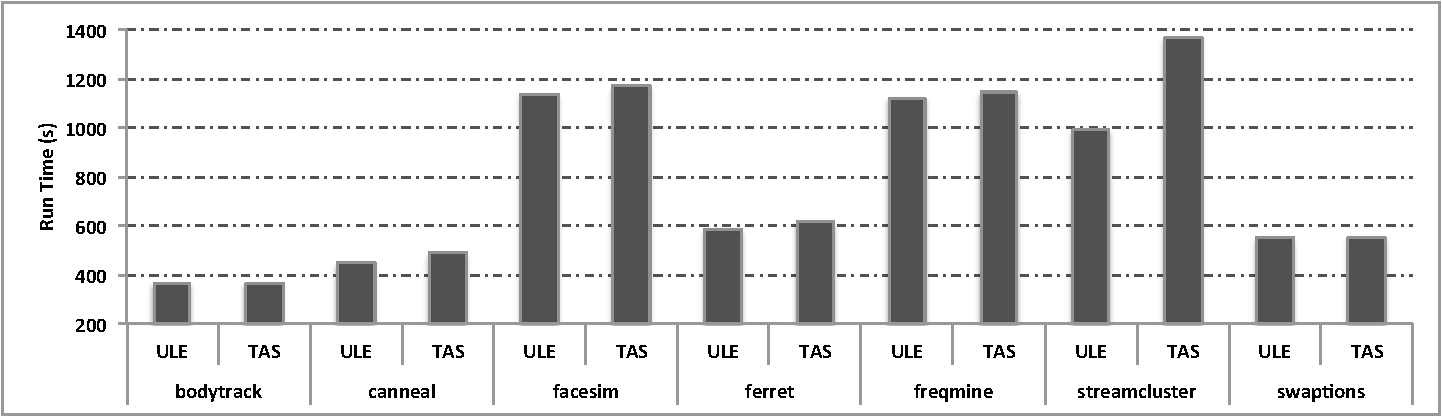
\includegraphics[width=1.0\linewidth,height=2.5in]{parsecperformance}
  \caption{Comparison of PARSEC benchmark performance under ULE and TAS
schedulers.}
  \label{fig:pbenchmarkp}
\end{figure} 
\begin{figure}[tbp]
  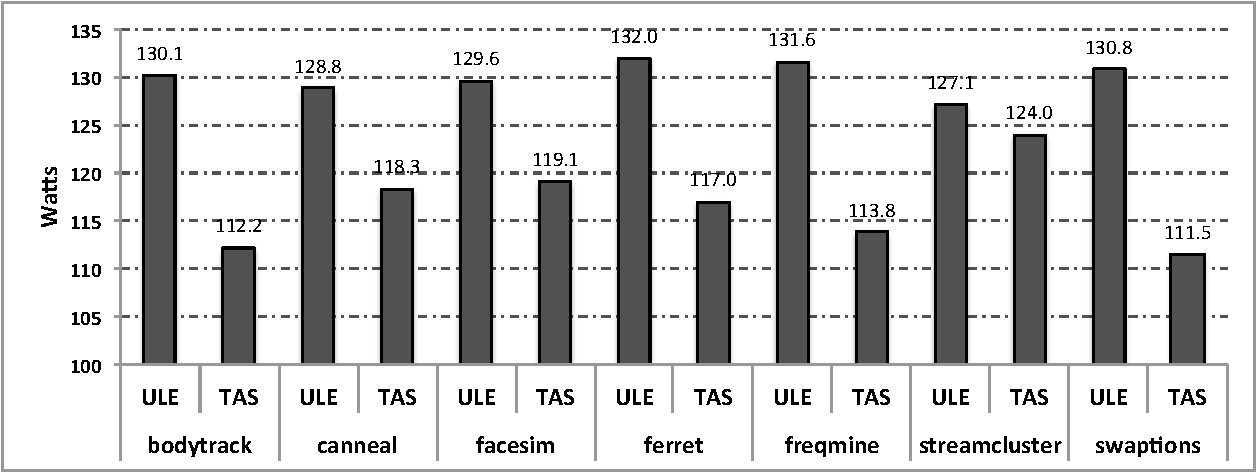
\includegraphics[width=1.0\linewidth,height=2.5in]{ParsecPowerConsumption}
  \caption{Comparison of PARSEC benchmark average power dissipation under ULE and TAS schedulers.}
  \label{fig:pbenchmark}
\end{figure}
\begin{figure}[tbp]
  \centering
  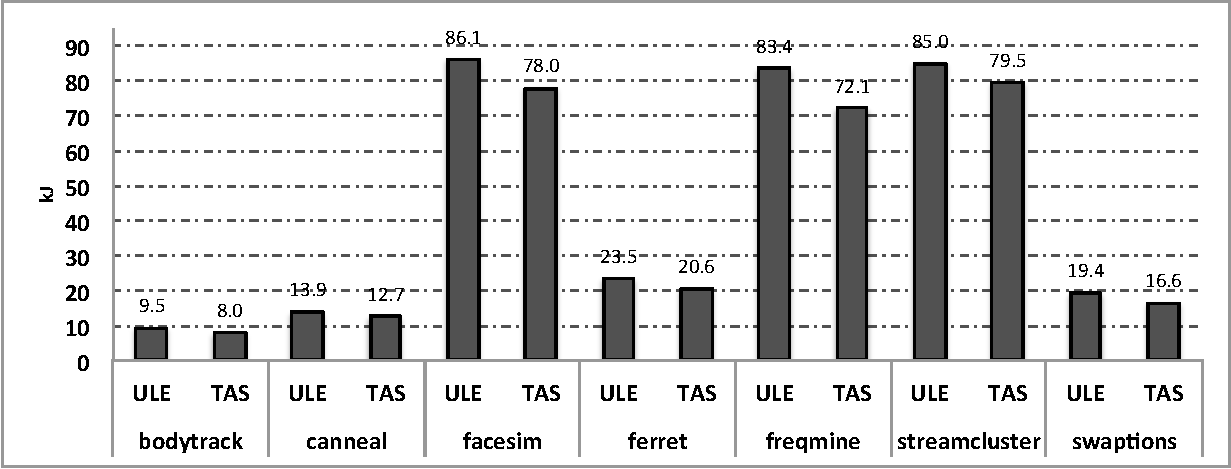
\includegraphics[width=1.0\linewidth,height=2.5in]{parseckj}
  \caption{Comparison of PARSEC total energy consumption under ULE and TAS schedulers.}
  \label{fig:penergy}
\end{figure}
Mean system power dissipation for each of the PARSEC benchmarks run on
our testbed under both schedulers is shown in
\figurename~\ref{fig:pbenchmark}.  When compared with ULE, TAS is
observed to reduce power dissipation markedly, from 14W (for the
\texttt{ferret} benchmark) to 19W (for \texttt{swaptions}), due to their
relatively small working sets.  On the other hand, less reduction in
power dissipation is found for benchmarks with large working sets,
lowering power by the range of 3W (for \texttt{streamcluster} to 10W
(for \texttt{facesim}).  The total energy consumption for each of the
PARSEC benchmarks run on our testbed is shown in
\figurename~\ref{fig:penergy}.  In comparison with ULE, TAS is observed
to reduce energy consumption between 2.8kJ (for \texttt{ferret}) to
2.9kJ (for \texttt{swaptions}) for benchmarks with relatively small
working sets, resulting in 14\% to 17\% reduction.

% In \figurename~\ref{fig:tasvsedp}, we contrast the optimization strategy
% used by TAS versus other possible optimizations schemes for managing the
% trade-off between performance and energy.  In this figure, we compare
% the energy savings from TAS for \texttt{facesim} benchmark to schemes
% that minimize delay under peak power constraints (DPC) and minimize
% energy under peak power and delay constraints (EPDC). DPC minimizes the
% delay of an execution interval so that the maximum power within an
% execution interval never exceeds a limit while EPDC schemes seek to
% minimize energy while operating a system within a power budget with a
% limit on the workload performance impact.  For the TAS results, we have
% integrated the mean power dissaption over time to compute energy use to
% compute percentage energy savings and compare against results reported
% in prior work~\cite{Cochran2011}. In this case, the optimizations used
% by TAS outperforms both DPC and EPDC for the \texttt{facesim} benchmark
% by 4\% to 6\% (against reported results in prior work of mean system
% power dissipation of 108W to 115W on a quad-core Intel processor).

% \begin{figure}[bpt]
%   \centering
% 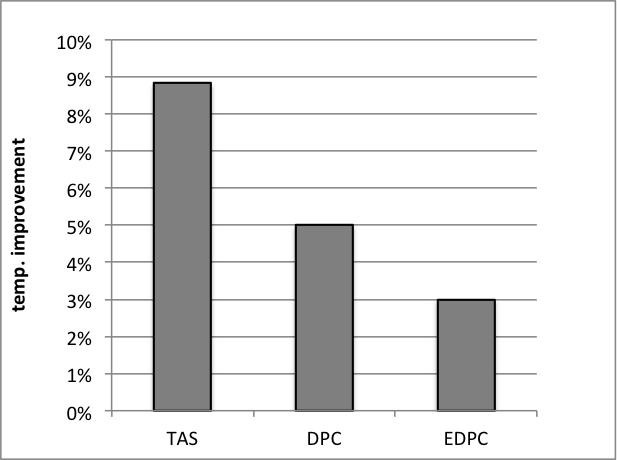
\includegraphics[width=1.0\linewidth,height=1.3in]{graphics/tasvsedpc}
%   \caption{Average percentage reduction in core die temperature for the
%     \texttt{facesim} benchmark under various optimization strategies.}
%   \label{fig:tasvsedp}
% \end{figure}
% \begin{comment}
%   Last sentence should be revised and extended per last sentence in
%   introduction. 
% \end{comment}

% Following comment block used by GNU-EMACS and AUCTEX packages
% Please do not remove.
%%% Local Variables: 
%%% mode: latex
%%% TeX-master: "dissertation.tex"
%%% TeX-PDF-mode: t
%%% TeX-source-correlate-mode: t
%%% End: 

%
% File:        chapter-conclusions.tex
% Author:      awl8049
% Revision:    $$
%
\chapter{Conclusions}
\label{chp:conclusions}
A fast and accurate model for energy consumption and thermal envelope in
a server is critical to understanding and solving the power management
challenges unique in dense servers.  In this work, we have introduced a
comprehensive model of energy consumption by servers as a continuous
system of differential equations.  The model measures energy input to
the system as a function of the work done for completing tasks being
gauged and the residual thermal energy given off by the system as a
result.  Traffic on the system bus, misses in the L2 cache, CPU
temperatures, and ambient temperatures are combined together to create a
model, which can be employed to manage the processor thermal envelope.

The model serves as a predictive tool by approximating observed
performance metrics in a discrete time series for estimating future
metrics, and thus corresponding energy consumption amounts.  It was
found through experimental validation that commonly used techniques of
regressive time series forecasting, while attractive because of their
simplicity, inadequately capture the non-linear and chaotic dynamics of
metric readings for typical server systems.  Therefore, a chaotic time
series approximation for run-time power consumption is adopted to arrive
at Chaotic Attractor Prediction (CAP), which exhibits polynomial time
complexity.  Our proposed model is the first step towards building
solutions for power and thermal management in data centers usually
housing many servers.

Dense servers pose power and thermal challenges, which often cannot be
addressed satisfactorily by conventional DVFS and DTM mechanisms,
especially under heavy workloads common for high-performance systems.
We have investigated into thermal-aware scheduling to deal with such
challenges, capable of managing system energy consumption within a given
power and thread envelope effectively.  As opposed to prior work aiming
to bound temperatures below critical thresholds, our proposed scheduler
considers how to dispatch heavy workloads in the high-performance
multi-core system for die temperature management across all cores.  It
is based on the thermal Chaotic Attractor Predictors (tCAPs) we develop
to guide thread selection and load balancing, taking into account key
thermal indicators and system performance metrics for preventing DTM
instances proactively.  The proposed tCAP-oriented scheduling (dubbed
the TAS scheduler) has been implemented to replace the original
scheduler of the FreeBSD operating system (called the ULE scheduler) for
evaluation on a testbed server under benchmarks from the SPEC CPU2006
and PARSEC suites.  Experimental results demonstrate that our TAS
scheduler can lower the mean on-die core temperature by up to
12.8$^{\circ}$C (from 44.8$^\circ$C down to 32.0$^\circ$C) under PARSEC
benchmarks and by up to 3.3$^{\circ}$C under mixes of SPEC benchmarks
for concurrent execution, while exhibiting negligible performance
degradation, in comparison to the ULE scheduler.  When compared with a
recent energy-aware scheduling technique reported to attain core
temperature reduction by up to 4$^\circ$C (from 63$^\circ$C down to
59$^\circ$C) upon executing four parallel scientific applications
compatible to PARSEC benchmarks on an Intel Xeon 5520 4-core processor
\cite{Sarood2011}, our TAS clearly enjoys better thermal reduction under
multi-threaded execution.

\section{Future Directions}
\label{sec:future-directions}
The topics of power and thermal management in large scale computing have
only recently begun to receive systematic attention.  Our work serves as
a starting point for a longer-term research program to consider some
unanswered question related to these topics.

The experimental validation of CAP reveals opportunities for further
investigation of power modeling. The model developed in this work is
valid for any dual-core/dual-processor system using NUMA memory access
connected in a point-to-point manner using the HyperTransport or the QPL
structures.  However, it can be scaled to quad-core dual processors
based on those two structures.  One would expect to see a slight
difference or variation in power prediction due to a greater or less
affect of die temperatures on the other performance measures.  Under a
dual-core quad-processor server, for example, additional regression
variables would be incorporated in $E_{proc}$, giving rise to more
performance measures (i.e., a larger $r$).  Similarly, more PeCs related
to cache misses would then be involved in $E_{mem}$.  The solution
approach of CAP remains exactly identical, except for a larger $r$ in
its prediction computation.  CAP has been validated for NUMA-based
servers, built on AMD Operton processors and Intel Xeon processors with
Nehalem architecture; it requires validation on other architectures,
like NVIDA GPU processors and IBM Cell BE processors.  Further studies
on the power and thermal envelope of multi-chip server systems, which
involve network traffic and off-chip synchronization traffic, is
required to understand their contributions to the system thermal
envelope.

Operating system schedulers such as the FreeBSD ULE scheduler were
introduced before the wide-spread adoption of multi-core processors such
as those used in our evaluation.   Thus, their scheduling decisions rarely
take into account the interactions within multi-core processors that
arise from contention of shared resources.   At best, as we have seen
with our extensions to push migration in TAS, they make very
coarse-grain decisions about how to address such resource contention.
For instance, recent studies ~\cite{McCullough2011}
identified that many methods used for power modeling suffer high
prediction errors due to inherent complexities of multiple cores, hidden
device states, and large dynamic power components.  The question of how
such errors impacts scheduling decisions has yet to be explored for both
existing schedulers and energy/thermal aware schedulers such as TAS.

Our Thermal Aware Scheduler considers scheduling only within a single
server blade. High-performance computing applications distribute
workload across multiple environments using interfaces such as MPI and
OpenMP.  A topic for further research is how to extend the CAP and
Thermal Aware Scheduling into such environments.   A recent study of
power profiles of a four-node cluster executing  MapReduce-style
codes~\cite{DavisRivoire2011} found that inter-node variability in
homogeneous clusters leads to substantially different single-node models
with higher error rates for cluster level measurements.  This study
shows the need to carefully consider the dynamics of the interactions
between nodes and tools like our chaotic attractor predictors are
well-positioned as a predictive tool for use in this use-case scenario.

A related topic is consideration of the effect of operating-system
virtualization on Thermal Aware Scheduling.  Some attention has been
applied to this area in recent work \cite{Merkel2010} but questions
remain open considering issues of scheduler interference between host
and virtual operating systems and the impact of virtualization on
power management in the clustered, grid, and cloud environment.  Open
questions remain as to how a scheduler in the virtual machine manager
coordinates energy and thermal management decisions with an operating
system in a virtual machine that is unaware of the virtual environment.
Scheduling decisions made within the virtual machine may lead to
unexpected contention for resources in use by other virtual machines
with unexpected consequences for thermal management.
% Following comment block used by GNU-EMACS and AUCTEX packages
% Please do not remove.
%%% Local Variables: 
%%% mode: latex
%%% TeX-master: "dissertation.tex"
%%% TeX-PDF-mode: t
%%% TeX-source-correlate-mode: t
%%% End: 

\bibliography{dissertation.bib}                      
% \index{Bibliography@\emph{Bibliography}}
%
% Generate the index.
%
%\printindex     % Include the index here. Comment out this line      %
%               % with a percent sign if you do not want an index .  %
 \begin{abstract} 
   Modern processors crudely manage thermal emergencies through Dynamic
   Thermal Management (DTM), where the processor monitors the die
   temperature and dynamically adjusts the processor voltage and
   frequency (DVFS) to throttle down the processor when
   necessary. However, DVFS tends to yield marked degradation in both
   application performance and system reliability.  This dissertation
   proposes a run-time model relating server energy consumption to
   its overall thermal envelope, using hardware performance counters and
   experimental measurements.  Our approach differs from prior work by
   linking system energy input to subsystem energy consumption based on
   a small set of tightly correlated parameters.  The proposed model
   takes into account processor power, bus activities, and system
   ambient temperature for real-time prediction of the power consumption
   of long running jobs.  Using the HyperTransport and QuickPath Link
   structures as case studies and through electrical measurements on
   example server subsystems, we develop a chaotic time--series
   approximation for run-time power consumption, arriving at the Chaotic
   Attractor Predictor (CAP).  With polynomial time complexity, CAP
   exhibits high prediction accuracy, with prediction errors within
   1.6\% (or 3.3\%) for servers based on the HyperTransport bus (or the
   QuickPath Links), as verified by a set of common processor
   benchmarks.

   Based on our Chaotic Attractor Predictors, we have developed and
   evaluated an effective thread scheduler for multi-core systems.
   Besides CAPs, our scheduler uses two basic principles to minimize
   server energy consumption: (1) selecting the thread with the least
   probability of causing a DTM in the subsequent time quantum, for
   execution on the next available core, and (2) migrating execution
   threads on thermally overextended cores to other cool cores via load
   balancing.  Our scheduler is evaluated in practice to assess the
   advantages resulting from incorporating thermal-awareness into the
   existing scheduler in the FreeBSD operating system.  Experiments
   reveal that our scheduler exhibits reduction in mean core on-die
   temperatures by up to 12.8$^{\circ}$C\ under PARSEC benchmarks (which
   have multi-threaded workloads) and by up to 3.3$^{\circ}$C\ under
   mixes of SPEC CPU2006 benchmarks for concurrent execution on all four
   server cores, while experiencing only 1\% to 4\% performance
   degradation.
 \end{abstract}

\begin{biography}
  Adam Wade Lewis received a Bachelor of Arts in Mathematics and
  a Bachelor of Arts in Theatre from the The University of the
  South in 1986 and a Master of Science in Computer Science from
  The University of Tennessee at Chattanooga in 1989. His background
  includes experience in the retail information technology and
  networking engineering fields as a Software Developer, Business
  Analyst, and Project Manager for NCR~Corporation throughout the
  world. He is a member of SIAM, the ACM, and the IEEE Computer Society.
 \end{biography}


\end{document}
% The following comment block is used by the different flavors of EMACS and
% the AUCTEX package to manage multiple documents.  In order for AUCTEX
% to understand you're working with multiple files, you should define
% the TeX-master variable as a file local variable that identifies your
% master document.
%
% Please do not remove.
%%% Local Variables: 
%%% mode: latex
%%% TeX-master: "dissertation.tex"
%%% TeX-PDF-mode: t
%%% TeX-source-correlate-mode: t
%%% End: 
